\documentclass{article}

\usepackage{iclr2027_conference,times}

\input{math_commands.tex}

\usepackage{url}
\usepackage{tikz}
\usetikzlibrary{shapes.geometric}
\usepackage{pgfplots}
\usepackage{float}
\usepackage{hyperref}
\pgfplotsset{compat=1.18}
\usepackage{xcolor}
\usepackage{booktabs}
\usepackage{fvextra}
\usepackage{graphicx}
\usepackage{enumitem}



% Okabe-Ito Colorblind-Friendly Palette (5 Distinct Curves)
\definecolor{CBPurple}{HTML}{CC79A7} % GPT-5-mini
\definecolor{CBBlue}{HTML}{0072B2}   % DeepSeek-V4-Pro
\definecolor{CBOrange}{HTML}{D55E00} % DeepSeek-V4-Flash
\definecolor{CBGreen}{HTML}{009E73}  % Qwen3-235B-A22B
\definecolor{CBRed}{HTML}{E69F00}    % Llama-3.3-70B-Instruct
\title{ARCUS-X: Adaptive Rule Compliance Under Sequential eXecution for Diagnosing Long-Horizon Language Model Reliability}

\author{Anonymous Authors}

\begin{document}
\maketitle

\begin{abstract}
Long-horizon language-model evaluations often reduce performance to final-answer accuracy, obscuring failures that accumulate across dependent sequential transitions. We introduce ARCUS-X, an auditable benchmark and evaluation protocol for decomposing deterministic sequential execution into trajectory correctness, continuity, rule binding, horizon control, response validity, and excess generation. ARCUS-X uses procedurally generated toroidal-grid tasks with exact per-transition ground truth, controlled lexical and transition perturbations, raw-stream preservation, and deterministic post-run diagnostics. Across 13 models, ARCUS-X exposes substantial separation between aggregate trajectory quality and observed failure signatures. In the adaptively sampled runs, GPT-5-mini attains 85.3\% step accuracy, 36.0\% exact match, and 85.0\% continuity, but 25.6\% generation efficiency and 11.2\% invalid responses. Under the failure taxonomy, state-tracking signatures account for 94.0\% of valid Qwen 3 Coder 480B A35B probes and 84.3\% of valid GLM-5 probes, while Mistral Large 2512 has 24.8\% transition-rule signatures and Kimi K2.5 has 23.2\% semantic-interpretation signatures. Horizon signatures, including overlong outputs, account for 49.4\% and 56.1\% of valid Mistral Large and Kimi probes, respectively. Sampled fracture behavior also varies by perturbation tier. Because AFS allocates horizons from observed performance, pooled aggregates describe the acquired support rather than a common uniform horizon distribution. ARCUS-X therefore provides a reproducible diagnostic record of explicit state-transition execution rather than a universal model ranking or measure of general long-horizon agency.

\end{abstract}

\section{Introduction}

As large language models (LLMs) are increasingly used for complex scientific and software tasks, reliability over long sequences has become an important evaluation problem. Existing evaluations such as GSM8K \cite{cobbe2021gsm8k}, MMLU \cite{hendrycks2020mmlu}, and LiveBench \cite{gu2024livebench} primarily measure task-level correctness, while execution-based evaluations such as HumanEval \cite{chen2021evaluating} test functional correctness. These evaluations are useful for determining whether a task succeeds, but they provide limited information about how reliability changes as dependent intermediate states accumulate across a sequence.

This becomes important when two models achieve similar final outcomes but fail in fundamentally different ways. One may gradually drift from the correct state, while another may preserve the state but fail to terminate correctly. Final-answer metrics can therefore hide behaviors such as state drift, incorrect intermediate transitions, horizon-dependent degradation, and failures to preserve constraints throughout execution.

Recent work has begun to study reliability across longer executions and through trajectory-level analysis. \textit{Beyond pass@1} \cite{khanal2026pass1reliabilityscienceframework} examines reliability as task duration increases, while \textit{Long-Horizon Agent Trajectory Attribution} \cite{chen2026longhorizonagenttrajectoryattribution}, AgentRewardBench \cite{lu2025agentrewardbench}, Plan-RewardBench \cite{wang2026aligning}, and KellyBench \cite{grady2026kellybench} study long-horizon behavior through trajectories, rewards, attribution, and sequential decision making. ARCUS-X complements this work by focusing on a narrower unit of analysis: \textbf{sequential state-transition execution}. Rather than evaluating an entire agent environment, ARCUS-X uses procedurally generated deterministic tasks where each transition has deterministically computable ground truth, independent from model evaluation. This allows horizon and semantic perturbations to be controlled directly while measuring how reliably models maintain and transform state over time.

To address this, we introduce ARCUS-X as an auditable benchmark and evaluation protocol for long-horizon sequential execution. ARCUS-X evaluates the trajectory rather than only its final outcome, characterizing state preservation, rule binding, perturbation robustness, horizon control, sampled fracture behavior, validity, and output overhead. Its central object is diagnostic decomposition: similar aggregate accuracy can conceal different observable signatures, including state drift, rule misapplication, rule-binding errors, premature termination, and formatting failure. ARCUS-X is designed not to introduce trajectory evaluation itself, but to assign reproducible behavioral signatures under controlled transitions, perturbations, operational validity, and an explicit precedence policy. These labels describe benchmark behavior, not hidden model cognition.

This work makes the following contributions:

\begin{enumerate}

\item We introduce ARCUS-X, an auditable, procedurally generated benchmark and evaluation protocol for sequential state-transition execution reliability.

\item We develop trajectory-level metrics and a deterministic diagnostic taxonomy that distinguish state tracking, transition-rule application, semantic interpretation, horizon collapse, and formatting without reducing reliability to a single accuracy value.

\item We provide controlled lexical and transition perturbations that probe rule binding separately from transition-system execution, together with a bounded AFS protocol that directs evaluation toward threshold-relevant horizons without exhaustively evaluating every horizon.

\item We report an auditable evaluation workflow with deterministic seeded probes, independently validated ground truth, raw-stream preservation, resumable evaluation, experiment metadata, and explicit separation of operational from cognitive failures.
\end{enumerate}

Code, evaluation artifacts, and reproducibility materials are available at \url{https://anonymous.4open.science/r/ARCUS-X}.


\section{Related Work}

Existing LLM evaluations such as GSM8K \cite{cobbe2021gsm8k}, MMLU \cite{hendrycks2020mmlu}, and LiveBench \cite{gu2024livebench} primarily measure task-level correctness, while HumanEval \cite{chen2021evaluating} evaluates functional correctness through execution-based tests. These benchmarks assess whether a task is completed, but they provide limited information about how reliability changes across dependent state transitions.

Recent work extends evaluation toward reliability and trajectory-level analysis. \textit{Beyond pass@1} \cite{khanal2026pass1reliabilityscienceframework} studies reliability as a function of task duration, including reliability decay, variance amplification, and meltdown onset. \textit{Long-Horizon Agent Trajectory Attribution} \cite{chen2026longhorizonagenttrajectoryattribution}, AgentRewardBench \cite{lu2025agentrewardbench}, and Plan-RewardBench \cite{wang2026aligning} further examine trajectory-level behavior, attribution, and evaluation.

\textit{The Illusion of Diminishing Returns} \cite{sinha2026execution} isolates long-horizon execution by supplying the knowledge and plan needed for a task, and studies how reliability changes with execution length. \textit{Reasoning or Reciting?} \cite{wu2024counterfactual} evaluates counterfactual task variants, including altered spatial conventions. ARCUS-X builds on these directions rather than claiming that execution-depth effects or rule perturbations are new in isolation.

RULER \cite{hsieh2024ruler} evaluates long-context capabilities through retrieval, multi-hop tracing, and aggregation tasks. LongMemEval \cite{wu2025longmemeval} evaluates long-term conversational memory, including information extraction, multi-session and temporal reasoning, knowledge updates, and abstention. LoCoMo \cite{maharana2024locomo} examines long-term conversational memory through multi-session interactions and associated reasoning tasks.

Broader agent benchmarks instead evaluate success in naturalistic, multi-step environments. SWE-bench \cite{jimenez2024swebench} evaluates repository-level issue resolution, WebArena \cite{zhou2024webarena} evaluates web-agent behavior, and AgentBench \cite{liu2024agentbench} spans multiple interactive environments. These settings deliberately combine planning, tool use, observation, and environment-specific uncertainty. ARCUS-X is not a substitute for them. Rather, it removes those factors to test whether a model follows an explicitly specified deterministic transition system. This controlled scope permits exact trajectory-level attribution, but does not establish general long-horizon agent capability or reliability across long-horizon agents. KellyBench \cite{grady2026kellybench} and related sequential decision-making environments provide additional tests of extended decision making.

ARCUS-X addresses a narrower evaluation objective than these long-context and memory benchmarks: the reliability of executing explicitly specified deterministic state transitions over dependent sequences. Rather than primarily testing retrieval or memory across extended contexts, ARCUS-X evaluates intermediate states against a computer-generated reference trajectory. Its contribution lies in jointly characterizing transition correctness, temporal continuity, exact trajectory agreement, horizon compliance, operational validity, and generation overhead under controlled rule perturbations. Long-horizon degradation and trajectory evaluation are not claimed as novel in themselves; the benchmark provides an auditable decomposition of observable sequential execution behavior.
\section{Methodology}

\label{Methodology}

ARCUS-X isolates long-horizon sequential execution reliability under controlled and deterministic perturbations.

\subsection{Experimental Design}

Within ARCUS-X, the base unit of evaluation is a probe:
a deterministic task instance defined by its initial
coordinate, grid dimensions, transition rules, ordered
action sequence, and requested trajectory length $z$.
The prompt requires exactly $z$ output coordinates,
including the initial state. The task generator supplies
$z$ actions, of which the first $z-1$ determine the
requested output trajectory.
\subsection{Procedural Generation of Probes}

ARCUS-X uses seeded procedural generation: the same seed and configuration regenerate the same probe. Unless a grid-size sweep is enabled, width $W$ and height $H$ are sampled independently and uniformly from $[5,12]$; initial coordinates and action sequences are deterministically sampled from the same probe seed. Horizon and perturbation tier are controlled separately. Each probe contains $z$ supplied actions, of which the first $z-1$ determine the requested output trajectory.

\subsection{Transition Rules and Environment}

ARCUS-X's environment is based on a grid defined as the formal state space. The state is represented as a coordinate $[x,y]$. The grid is two-dimensional, composed of a width, \textit{W}, and height, \textit{H}. The environment is toroidal; hence, crossing an edge wraps to the opposite side.

Each action corresponds to its labeled deterministic transition $(\Delta x, \Delta y)$. At each step, the model must first identify the action, retrieve its associated transition, apply it to the current state, and finally wrap the resulting coordinate. This wraparound behavior is implemented using a modulo operation. It is a sequential task because the next state entirely depends on the previous state.

\begin{align*}
    x_{t+1} &= (x_t + \Delta x_t) \mod W \\
    y_{t+1} &= (y_t + \Delta y_t) \mod H
\end{align*}

Coordinates are indexed from 0 to $W-1$ along the horizontal axis, and likewise from 0 to $H-1$ along the vertical axis.

\subsection{Perturbation Regimes}
\label{subsec:pert_regi}
ARCUS-X perturbs the model-facing task along a four-level categorical \emph{tier} axis (Tier 0--3). These tiers are the active perturbations analyzed here. Stored runs also contain a legacy semantic-gravity value $g$, but in the main runner $g$ neither alters the prompt nor selects the tier; all four tiers are crossed with each configured $g$. We therefore interpret results by tier, not $g$ as an independent semantic-difficulty variable.

\begin{enumerate}

    \item Tier 0 provides the baseline, in which there are standard directional labels and $(\Delta x, \Delta y)$ rules. Tier 0 establishes baseline state-tracking performance.

    \item Tier 1 is a semantic disruption tier. It renames action labels to pseudowords; however, the underlying transition structure remains unchanged. This tests whether the model can bind arbitrary labels to the explicitly given rules rather than relying on familiar words such as ``north'' or ``south.''

    \item Tier 2 is an attribute inversion tier, in which each transition is transformed as follows:

    $(\Delta x, \Delta y) \rightarrow (\Delta x, -\Delta y)$

    The ground truth is recomputed using the transformed rules. This tests whether the model follows the provided transition system rather than its prior assumptions about spatial directions.

    \item Tier 3 acts as a coordinate transformation tier. It transforms each transition using a $90^\circ$ rotation:

    $(\Delta x, \Delta y) \rightarrow (-\Delta y, \Delta x)$

    This tests whether the model can maintain the state-transition procedure when the spatial behavior conflicts with ordinary directional intuition. Ground truth is recomputed using the transformed transition rules.

\end{enumerate}

The prompt contains the assigned labels and rules, grid dimensions, initial state, action sequence, question, and required output format; it omits $g$, hidden answers, and difficulty metadata. Stored runs use $g\in\{0.5,3.0,15.0\}$ crossed with all four tiers; because $g$ is inert in this sweep, these values function as replicated configuration strata rather than semantic perturbations. Fixed calibration probes at $g=0.0$, $z=3$, Tier 1 are parsing/environment checks and are excluded from reported metrics.

\subsection{Evaluation}

We implement a native evaluation harness for ARCUS-X that separates probe generation, deterministic environment execution, model inference, response parsing, trajectory scoring, diagnostic classification, and adaptive fracture analysis. Model outputs are evaluated against independently computed ground-truth trajectories.

ARCUS-X records the model's trajectory, raw response, and inference metadata, including latency, output tokens, completion status, and provider/API errors. These measurements are independent of trajectory correctness, allowing execution, formatting, and efficiency failures to be distinguished from state-tracking errors. Responses are classified as valid trajectory, malformed recoverable output, empty output, parser failure, provider failure, or runtime/exception failure.

For a requested horizon $z$, the prompt explicitly requires
exactly $z$ output coordinates, including the provided initial
state. Accordingly, the evaluated reference trajectory is
defined as
\[
\mathbf{s}_0,\mathbf{s}_1,\ldots,\mathbf{s}_{z-1},
\]
where $\mathbf{s}_0$ is the initial state and $\mathbf{s}_t$
is the state reached after executing the first $t$ actions.

Although the task generator supplies $z$ action instructions,
only the first $z-1$ actions determine the requested output
trajectory. The final action does not correspond to a
requested output coordinate and is excluded from trajectory
scoring.

Step Accuracy and Continuity evaluate the $z-1$ post-initial
positions. Requested-output Exact Match requires equality across all $z$
requested coordinates, including the initial state. The post-hoc
taxonomy uses the same requested-output reference, while preserving the full
generated $z+1$-state trajectory for audit. Horizon Compliance
measures adherence to the specified output length $z$.

ARCUS-X calculates the following raw measurements:
\begin{enumerate}
    \item Output tokens: total generated tokens obtained from provider metadata or estimated, with source and benchmark confidence saved in raw output files.
    \item Output tokens per second.
    \item Correct transitions per second.
\end{enumerate}

ARCUS-X uses multiple master seeds generated via a TRNG utilizing atmospheric noise \cite{haahr_random_org}. Main tables report pooled probe-level means over the observations actually acquired by AFS. Because AFS may evaluate different horizon sets for different models and conditions, these pooled quantities are descriptive summaries of the observed support, not estimates under a shared uniform horizon distribution. Appendix~\ref{app:seed_variance} reports the population mean and standard deviation of CRI across the five master seeds; raw artifacts retain per-seed CRI and fracture depth. We do not claim statistical significance for between-model differences.

\subsection{Failure Taxonomy}
\label{subsec:failure_taxonomy}
The taxonomy is a deterministic post-scoring diagnostic, not an inference about a model's internal cognition. The post-hoc \texttt{classify\_requested\_output} entry point in \texttt{arcus/analysis/taxonomy.py} applies diagnostic precedence to the requested $z$-coordinate reference; Appendix~\ref{app:failure_taxonomy} specifies its decision rules. The label \emph{None} requires an operationally valid, exact requested-output match; perfect Step Accuracy alone is insufficient. Invalid responses do not enter the trajectory taxonomy, and valid unmapped cases are retained as \emph{unknown/unmapped}. These signatures describe observable outputs, not latent cognitive causes.

\subsection{Metrics}
\label{subsec:Metrics}

The primary measures of sequential execution reliability are:
\begin{enumerate}
    \item \textbf{Step Accuracy}
    \[
    \text{Step Accuracy} =
    \frac{\text{number of correctly reproduced post-initial states}}
    {z-1}.
    \]
    Comparison is performed at aligned post-initial positions over the
    overlapping region. The initial state is not counted. At $z=1$,
    no transitions are scored; the implementation records zero rather
    than interpreting this as evidence about transition execution.

    \item \textbf{Requested-output Exact Match}, which is binary per probe and requires identical coordinates and length against the first $z$ reference states. In the pooled tables its denominator is all completed non-calibration probes; invalid responses are nonmatches.

    \item \textbf{Continuity}, defined as the longest correct transition
    prefix:
    \[
    \text{Continuity} =
    \frac{\text{longest correct post-initial prefix}}
    {z-1}.
    \]
\end{enumerate}

First divergence is reported as a diagnostic rather than a primary aggregate metric. It records the 1-based position of the first mismatch; if the overlapping region is correct but the lengths differ, divergence is assigned to the first position beyond the overlap.

ARCUS-X also measures horizon and output behavior:
\begin{enumerate}
    \item \textbf{Horizon Compliance}
    \[
    \text{HC} =
    1 -
    \frac{\left|L_{\mathrm{pred}}-z\right|}
    {\max(L_{\mathrm{pred}},z)}.
    \]

    \item \textbf{Generation Bloat Index}
    \[
    \text{GBI} =
    \frac{\max(0,T_{\mathrm{actual}}-T_{\mathrm{expected}})}
    {T_{\mathrm{expected}}},
    \]
    where $T_{\mathrm{actual}}$ is the completion-token count. The deterministic completion allowance is $T_{\mathrm{expected}}=10z+10$: ten tokens for each of the $z$ coordinate pairs plus a ten-token formatting allowance. GBI therefore measures \emph{excess generation relative to this fixed benchmark allowance}; it is not a tokenizer-invariant minimum-description-length estimate. Provider usage is used when available; otherwise token counts fall back, in order, to an official tokenizer, a compatible tokenizer, or a documented deterministic heuristic. Token source and confidence are retained per probe.

    \item \textbf{Generation Efficiency}
    $\text{GE} = \frac{1}{1+\text{GBI}}$ per probe. Reported GE and GBI columns are each arithmetic means of their respective per-probe values; consequently, mean GE is not generally equal to $1/(1+\text{mean GBI})$.
\end{enumerate}

We additionally report the Composite Robustness Index (CRI) as a secondary, researcher-specified composite of trajectory fidelity, horizon robustness, perturbation robustness, and generation efficiency. Its formulation and fixed weights are provided in Appendix~\ref{app:CRI}; primary claims in this paper rely on the decomposed measurements rather than CRI alone.

ARCUS-X also reports system-level efficiency using latency. Latency is total wall-clock response time and is treated as a systems-level diagnostic because it depends on batching, deployment conditions, and provider infrastructure: $\text{ALE} = \text{Accuracy}/\text{Latency}_{\mathrm{seconds}}$.
\subsection{Adaptive Fracture Search}

Adaptive Fracture Search (AFS) is a bounded, reproducible, threshold-directed allocation protocol that acquires observations near horizons where valid-response step accuracy falls below a 50\% floor without scanning every integer horizon.

The search uses accuracy over all $z$ action transitions, whereas the reported trajectory metrics evaluate the first $z-1$ transitions. At each horizon $z$, cognitive step accuracy is computed over operationally valid trajectories: $A(z)=\frac{1}{|V_z|}\sum_{i\in V_z} a_i$,

where $V_z$ is the set of analyzable probes and $a_i$ is the step accuracy of probe $i$. Operational failures are excluded from $A(z)$ and reported separately. Accordingly, $A(z)$ is conditional accuracy given an analyzable trajectory; it should not be interpreted as end-to-end success when validity itself declines.

AFS evaluates midpoint horizons with a bisection-style controller and expands its upper bound while performance remains above the floor. The controller is an allocation heuristic, not a monotonic-capacity model: recoveries remain visible in the sampled curve and are handled post hoc. Invalid or infrastructure-failed responses are excluded from the batch mean; a batch with no valid observations is operationally insufficient evidence. Evaluated probes are cached and reused.

The live-search value $z^{*}$ is a below-floor horizon encountered by the allocation procedure, or a censored ceiling outcome when none is observed; it is not guaranteed to be the first failing horizon. A separate forward-look-ahead analysis reports \emph{sampled structural fracture}. Both operate on adaptively sampled points, so fracture values are condition-specific diagnostics of the acquired curve rather than intrinsic capacities. The configured ceiling is $z=150$.

A controlled synthetic comparison of sampling policies is reported in Appendix~\ref{app:afs_simulation}.
\section{Results}

\subsection{Benchmark Performance}
We evaluate ARCUS-X on 13 models and focus the detailed analysis on the five representative models in Table~\ref{tab:overall_results}; the Appendix reports all 13. The representative set uses fixed Generally Available model versions: GPT-5-mini (Microsoft Azure Foundry, version 2025-08-07), Kimi K2.5 (AWS Bedrock), GLM-5 (AWS Bedrock), Qwen 3 Coder 480B A35B (AWS Bedrock), and Mistral Large 2512 (Mistral AI API). Runs used five probes per evaluated batch, five master seeds, and temperature 0 or the lowest allowed value. Because AFS evaluates model- and condition-dependent horizon sets, completed execution counts and horizon mixtures differ across runs; the exact matrix is retained in each manifest and raw artifact. Unless explicitly conditioned on a shared horizon, the pooled values below therefore compare the observed AFS-supported samples and should not be read as estimates over an identical horizon distribution.
\begin{table}[!ht]
\centering
\caption{Overall ARCUS-X trajectory-level performance over all recorded non-calibration probes. Exact Match uses the requested $z$ coordinates and all completed probes; taxonomy \emph{None} uses the same exact-match condition among valid responses. Asterisks indicate response validity below 75\%. Validity denotes the proportion of probes yielding cognitively analyzable responses.}
\label{tab:overall_results}
\scriptsize
\resizebox{\linewidth}{!}{%
\begin{tabular}{lccccc}
\toprule
\textbf{Model} & \textbf{Step Acc.} & \textbf{Requested Exact Match} & \textbf{Continuity} & \textbf{Horizon Compliance} & \textbf{Validity} \\
\midrule
GPT-5-mini & 85.3\% & 36.0\% & 85.0\% & 87.7\% & 88.8\% \\
Kimi K2.5 & 59.2\% & 0.1\% & 53.9\% & 77.0\% & 94.8\% \\
GLM-5 & 56.2\% & 1.0\% & 51.3\% & 98.4\% & 100.0\% \\
Qwen 3 Coder 480B A35B & 49.7\% & 1.2\% & 43.1\% & 98.3\% & 100.0\% \\
Mistral Large 2512 & 56.0\% & 0.4\% & 53.0\% & 45.2\% & 96.9\% \\
\bottomrule
\end{tabular}}
\end{table}
Within the observed AFS-supported pools, GPT-5-mini has the highest step accuracy, exact match, and continuity of the five representative runs: 85.3\% step accuracy, 36.0\% exact match, and 85.0\% continuity. The other four show 49.7--59.2\% step accuracy and 0.1--1.2\% exact match. GLM-5 and Qwen 3 Coder 480B A35B also show that high horizon compliance can coexist with lower trajectory correctness. These are run-level descriptive comparisons, not a controlled ranking over matched horizons.

\subsection{Horizon-Dependent Degradation and Fracture}
\begin{figure}[!ht]
\centering
\begin{minipage}[c]{0.94\linewidth}
\centering
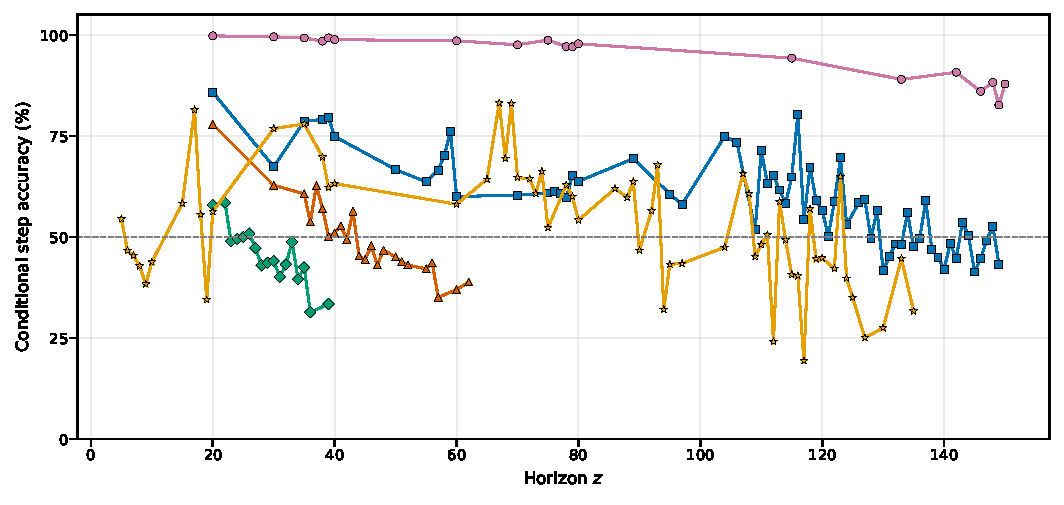
\includegraphics[width=\linewidth]{horizon_profiles_selected_valid_only.pdf}
\end{minipage}
\vspace{-2pt}
\begin{center}
\scriptsize
\setlength{\tabcolsep}{5pt}
\begin{tabular}{@{}llll@{}}
\tikz[baseline=-0.6ex]{\draw[CBPurple, line width=0.7pt] (0,0) -- (0.34,0);
  \node[circle, fill=CBPurple, draw=black, line width=0.3pt, minimum size=4.4pt, inner sep=0pt] at (0.17,0) {};} &
GPT-5-mini &
\tikz[baseline=-0.6ex]{\draw[CBBlue, line width=0.7pt] (0,0) -- (0.34,0);
  \node[rectangle, fill=CBBlue, draw=black, line width=0.3pt, minimum size=4.4pt, inner sep=0pt] at (0.17,0) {};} &
Kimi K2.5 \\[2pt]
\tikz[baseline=-0.6ex]{\draw[CBOrange, line width=0.7pt] (0,0) -- (0.34,0);
  \node[regular polygon, regular polygon sides=3, fill=CBOrange, draw=black, line width=0.3pt, minimum size=5pt, inner sep=0pt] at (0.17,0) {};} &
GLM-5 &
\tikz[baseline=-0.6ex]{\draw[CBGreen, line width=0.7pt] (0,0) -- (0.34,0);
  \node[diamond, fill=CBGreen, draw=black, line width=0.3pt, minimum size=4.6pt, inner sep=0pt] at (0.17,0) {};} &
Qwen 3 Coder 480B A35B \\[2pt]
\tikz[baseline=-0.6ex]{\draw[CBRed, line width=0.7pt] (0,0) -- (0.34,0);
  \node[star, star points=5, fill=CBRed, draw=black, line width=0.3pt, minimum size=5pt, inner sep=0pt] at (0.17,0) {};} &
Mistral Large 2512 &
\tikz[baseline=-0.6ex]{\draw[gray, dashed, line width=0.7pt] (0,0) -- (0.34,0);} &
50\% floor
\end{tabular}
\end{center}
\caption{Per-horizon step accuracy conditional on valid, non-calibration responses for the five representative models. Invalid-only horizons are omitted rather than assigned zero accuracy; lines connect only sampled horizons. Each sampled point is drawn with a model-specific marker (circle, square, triangle, diamond, or star) in addition to its color, so the curves remain distinguishable in grayscale.}
\label{fig:selected_models_horizon}
\end{figure}

Figure~\ref{fig:selected_models_horizon} shows conditional per-horizon step accuracy on the observed, nonuniform support. Profiles vary across models and are not uniformly monotone; lines connect sampled points for readability and do not interpolate missing horizons. Because AFS allocates probes adaptively (Appendix~\ref{app:afs_sampling}), the figure is a descriptive summary of valid-response performance rather than an estimator of a monotone capacity boundary.

\begin{table}[!ht]
\centering
\caption{Post-hoc structural fracture depth by perturbation tier for the five representative models, computed from valid non-calibration responses only. Values are the first sampled horizon below the 50\% conditional Step Accuracy floor without recovery in the next two sampled horizons. `N/A' means that no persistent sampled fracture was found; $\dagger$ marks a terminal candidate with insufficient look-ahead and is not a confirmed fracture.}
\label{tab:fracture_selected}
\scriptsize
\begin{tabular}{lcccc}
\toprule
\textbf{Model} & \textbf{Tier 0} & \textbf{Tier 1} & \textbf{Tier 2} & \textbf{Tier 3} \\
\midrule
GPT-5-mini & N/A & N/A & N/A & N/A \\
Kimi K2.5 & 145 & N/A & 130 & 55 \\
GLM-5 & 57 & 44 & 56 & 30 \\
Qwen 3 Coder 480B A35B & 34 & 24 & 28 & 23 \\
Mistral Large 2512 & 9 & 5 & 94 & 6 \\
\bottomrule
\end{tabular}
\end{table}

Table~\ref{tab:fracture_selected} shows that sampled structural fracture is strongly condition-dependent rather than an invariant model property. GPT-5-mini has no post-hoc fracture in the sampled curves, whereas Kimi K2.5 has late sampled fractures in Tier 0 and Tier 2 but an earlier one in Tier 3. Mistral Large 2512 makes the non-monotonicity especially clear: its Tier-2 sampled fracture is late despite much earlier values in the other tiers. The recovery rule operates on the next two \emph{sampled} horizons, whose spacing is not uniform, so these values describe the acquired curves rather than a fixed-width horizon neighborhood. The live AFS window was capped at $H=150$; reaching that cap without a below-floor midpoint is recorded separately as a saturated, right-censored result.

\subsection{Semantic Robustness}
As described in Section~\ref{subsec:pert_regi}, the benchmark runner evaluates all four perturbation tiers at each stored gravity configuration. Table~\ref{tab:tier_selected} reports per-tier step accuracy pooled over the observations acquired for each tier. Because AFS may sample different horizon mixtures across tiers, these values establish that the model-facing transformations produce distinct observed profiles, but they do not by themselves isolate a causal tier effect at matched horizons.

\begin{table}[!ht]
\centering
\caption{Per-tier step accuracy for the five representative models. Tier 0 is baseline; Tier 1 renames action labels only; Tier 2 inverts the $y$-delta; Tier 3 rotates transitions $90^\circ$.}
\label{tab:tier_selected}
\scriptsize
\begin{tabular}{lcccc}
\toprule
\textbf{Model} & \textbf{Tier 0} & \textbf{Tier 1} & \textbf{Tier 2} & \textbf{Tier 3} \\
\midrule
GPT-5-mini & 88.0\% & 83.7\% & 87.5\% & 82.2\% \\
Kimi K2.5 & 63.1\% & 75.8\% & 65.2\% & 32.9\% \\
GLM-5 & 64.5\% & 58.7\% & 60.3\% & 41.3\% \\
Qwen 3 Coder 480B A35B & 56.9\% & 49.7\% & 53.7\% & 38.4\% \\
Mistral Large 2512 & 56.1\% & 48.6\% & 58.6\% & 60.5\% \\
\bottomrule
\end{tabular}
\end{table}

The observed tier profiles are not ordered uniformly across models. GPT-5-mini spans 5.8 points between its highest and lowest pooled tier values. Kimi K2.5 and GLM-5 are substantially lower in Tier 3 than Tier 0 (30.2 and 23.2 points), while Qwen 3 Coder 480B A35B differs by 18.5 points. Mistral Large 2512 instead has its lowest pooled accuracy in Tier 1 and its highest in Tier 3, and Kimi K2.5 is higher in Tier 1 than Tier 0. These results argue against treating perturbation robustness as a single ordinal scalar: lexical relabeling and transition-altering transformations can produce different signatures for the same model. Because horizons are not matched by construction, we describe these as pooled tier associations rather than attributing the differences uniquely to the perturbation itself. Appendix~\ref{app:full_model} reports all 13 models and the CRI decomposition.

\subsection{Generation Efficiency and Failure Modes}
Aggregate trajectory accuracy does not capture output overhead. We therefore report Generation Efficiency (GE), derived from GBI, as a benchmark-relative excess-generation score and Correct Steps per Second (CSS) as a secondary systems measure; latency and output-token throughput remain supporting diagnostics (Section~\ref{subsec:Metrics}).
\begin{table}[!ht]
\centering
\caption{Generation efficiency measurements for the five representative models.}
\label{tab:generation_efficiency_selected}
\scriptsize
\begin{tabular}{lcccr}
\toprule
\textbf{Model} & \textbf{Step Accuracy} & \textbf{GBI} & \textbf{Generation Efficiency} & \textbf{Correct Steps/sec} \\
\midrule
GPT-5-mini & 85.3\% & 4.25 & 25.6\% & 1.922 \\
Kimi K2.5 & 59.2\% & 1.12 & 55.9\% & 2.406 \\
GLM-5 & 56.2\% & 0.00 & 100.0\% & 4.626 \\
Qwen 3 Coder 480B A35B & 49.7\% & 0.02 & 99.4\% & 6.786 \\
Mistral Large 2512 & 56.0\% & 4.49 & 23.8\% & 1.127 \\
\bottomrule
\end{tabular}
\end{table}

ARCUS-X separates correctness from output overhead. GPT-5-mini combines high step accuracy with low GE, whereas GLM-5 and Qwen 3 Coder 480B A35B have near-100\% GE but lower step accuracy. GE measures generation relative to the fixed benchmark allowance: 100\% means only that output did not exceed that allowance, not tokenizer-independent optimality. CSS remains a provider- and deployment-dependent systems diagnostic and does not enter trajectory, fracture, GBI, or CRI scoring.

Table~\ref{tab:failure_taxonomy_selected} reports the complete diagnostic partition for the representative models. Taxonomy percentages use valid probes as their denominator and include \emph{None} (requested-output exact match) and \emph{Unknown / Unmapped}; validity is reported separately over all completed probes. The same match condition in Table~\ref{tab:overall_results} uses all completed probes as its denominator. Every row's taxonomy columns sum to approximately 100\% after rounding, and invalid responses are not assigned a trajectory-level failure signature. Because the categories are precedence-based, their relative frequencies describe how the deterministic classifier partitions observed trajectories rather than independently validated latent mechanisms.

\begin{table}[!ht]
\centering
\caption{Post-run validity and requested-output taxonomy partition for the five representative models. Taxonomy percentages are relative to valid probes; \emph{None} is requested-output Exact Match.}
\label{tab:failure_taxonomy_selected}
\scriptsize
\resizebox{\linewidth}{!}{%
\begin{tabular}{lccccccccc}
\toprule
\textbf{Model} & \textbf{Valid} & \textbf{Invalid} & \textbf{State} & \textbf{Transition} & \textbf{Semantic} & \textbf{Horizon} & \textbf{Format} & \textbf{Unknown} & \textbf{None} \\
\midrule
GPT-5-mini & 88.8\% & 11.2\% & 10.4\% & 0.1\% & 0.0\% & 49.0\% & 0.0\% & 0.0\% & 40.5\% \\
Kimi K2.5 & 94.8\% & 5.2\% & 10.7\% & 4.0\% & 23.2\% & 56.1\% & 5.9\% & 0.0\% & 0.1\% \\
GLM-5 & 100.0\% & 0.0\% & 84.3\% & 0.6\% & 0.0\% & 14.2\% & 0.0\% & 0.0\% & 1.0\% \\
Qwen 3 Coder 480B A35B & 100.0\% & 0.0\% & 94.0\% & 1.1\% & 0.0\% & 3.6\% & 0.0\% & 0.0\% & 1.2\% \\
Mistral Large 2512 & 96.9\% & 3.1\% & 11.1\% & 24.8\% & 10.2\% & 49.4\% & 4.1\% & 0.0\% & 0.4\% \\
\bottomrule
\end{tabular}}
\end{table}

\section{Discussion}
\subsection{Central Finding}
Our central finding is that sequential reliability is multi-faceted rather than reducible to one score. ARCUS-X jointly reports trajectory correctness, prefix persistence, horizon compliance, perturbation profiles, validity, and output overhead. The deterministic taxonomy is applied uniformly across the 13-model publication cohort under strict correctness and canonical-coordinate rules: Table~\ref{tab:failure_taxonomy_selected} gives the complete validity and failure-signature partition for the five representative models, and Table~\ref{tab:failure_taxonomy_full} and Figure~\ref{fig:failure_profiles} extend it to all 13 models.

The important separation is descriptive. In the observed AFS-supported samples, high trajectory accuracy does not imply low output overhead, high horizon compliance does not imply high trajectory accuracy, and two models with similar pooled accuracy can produce very different diagnostic partitions. At the same time, adaptive sampling means these pooled values are not controlled estimates over a common horizon distribution, and the precedence-based taxonomy is not a causal account of internal cognition. ARCUS-X is therefore strongest as an auditable decomposition of observed execution behavior under explicit deterministic rules.
\subsection{Practical Uses}
The practical value of this decomposition is diagnostic: it can distinguish observable failure profiles that aggregate accuracy alone cannot identify and help formulate targeted follow-up investigations. Continuity and first-divergence measurements can help localize where execution begins to deteriorate. Horizon compliance can identify trajectories that stop before the requested length or continue beyond it. Controlled rule perturbations can reveal sensitivity to action labels or transformed transition conventions. These measurements do not by themselves establish why a model fails, but they make the behavior to investigate more specific.

Table~\ref{tab:overall_results} illustrates this distinction. GLM-5 and Mistral Large 2512 have similar pooled step accuracy (56.2\% and 56.0\%, respectively), but differ in observed horizon compliance (98.4\% and 45.2\%). Because AFS adaptively acquires different horizon sets across models and conditions, this is a descriptive comparison over unmatched supports, not a controlled estimate of a model difference. The result motivates examining horizon behavior alongside step accuracy; it does not demonstrate that a particular intervention will improve either model.

Accordingly, ARCUS-X supports claims about diagnostic utility rather than intervention effectiveness. Its failure profiles can motivate hypotheses for targeted model improvement and guide subsequent evaluation, while establishing the effectiveness of any specific intervention remains future work.
\subsection{Limitations}
ARCUS-X is synthetic by design: it isolates state-transition execution rather than planning, tool use, memory retrieval, partial observability, changing environments, or irreversible actions, and therefore does not measure general long-horizon agency. Provider/API conditions, response validity, and systems latency may also affect comparisons.

The main empirical limitation is adaptive support. AFS samples horizons nonuniformly from earlier outcomes, so models and tiers can be pooled over different horizon mixtures; completed-probe counts range from roughly 2{,}200 to 7{,}600 per model. Cross-model and cross-tier aggregates are therefore descriptive over acquired support, not matched-horizon causal estimates. The post-hoc fracture rule likewise uses three subsequent sampled points with variable spacing, making fracture a property of the sampled condition rather than an intrinsic capacity.

AFS accuracy is conditional on operational validity: unanalyzable responses are excluded from $A(z)$ and reported separately, so long-horizon invalidity can produce insufficient cognitive evidence rather than a low cognitive score. The taxonomy is reproducible but precedence-based and not externally validated; GBI/GE depend on a fixed token allowance and provider/tokenizer accounting; and CRI uses researcher-specified weights. Alternative precedence policies substantially redistribute diagnostic labels, so category frequencies should be interpreted as policy-dependent descriptive partitions rather than uniquely identified failure mechanisms. Five probes per batch and five master seeds characterize variation descriptively, not inferentially. Beyond the retrospective matched-horizon analyses and synthetic consistency checks in the appendix, future work should conduct prospectively balanced, task-paired fixed-horizon evaluation, independent taxonomy validation, and evaluation in richer sequential environments.
\section{Conclusion}


ARCUS-X shows that trajectory correctness, operational validity, output overhead, horizon behavior, and the composition of observed errors can diverge substantially. Across the adaptively sampled runs, models differ not only in pooled accuracy but in where trajectories break, whether requested horizon is preserved, how often output remains analyzable, and which deterministic failure signatures valid errors receive. No single scalar represents all of these behaviors.

The contribution is therefore not a universal ranking or intrinsic ``maximum horizon,'' but an auditable diagnostic record: deterministic tasks and ground truth, raw responses, validity status, per-probe measurements, sampled horizon curves, and an exhaustive post-run partition. AFS directs probes toward threshold-relevant horizons while preserving non-monotonicity, censoring, and operational insufficiency rather than converting them into capacity claims. ARCUS-X measures execution of explicit deterministic state-transition systems under controlled perturbations; it does not establish general agency, naturalistic planning, or tool-use competence.


\subsection*{Generative AI Disclosure Statement}

In this work, we used generative AI tools for soundboarding, refining the mathematical metrics and hypotheses, providing feedback on the methodology, and interpreting the results as a cohesive qualitative story. We did not use generative AI tools to generate synthetic datasets, develop proofs, or perform translation; implementation methods were not applicable to this work. We also used generative AI tools to edit LaTeX tables and figures, create and edit code, outline the paper, draft implementation pseudocode for the appendix implementation, make claims accurate to the working codebase, summarize existing literature, and identify gaps in the implementation as it evolved. Generative AI tools were used to polish and improve the clarity and readability of the manuscript at large. We reviewed all AI-assisted work. LLM-generated code was reviewed and audited multiple times, and the authors verified all AI-assisted edits to the paper. We also conducted an independent literature review to complement the generated summaries. We take responsibility for the final content of this work, including text, claims, and artifacts produced with the aid of generative AI.

\subsection*{Reproducibility statement}
ARCUS-X is reproducible at the task-generation, evaluation, and artifact levels.
Tasks are generated procedurally from explicit master seeds. The same
$(\text{seed},\text{tier},\text{task index})$ deterministically produces the
same grid, initial state, actions, transition rules, label mapping, and
ground-truth trajectory. All task randomness is derived from
\texttt{random.Random}; tier transformations and their ground truth are
recomputed deterministically. The reference trajectory is produced by the
single transition implementation in \texttt{arcus/environment/grid.py}, and
\texttt{validate\_ground\_truth()} checks it independently of model output.
A stable SHA-256 experiment signature in the code release identifies
the generated task inputs; it is not itself a source-revision identifier. The available raw streams retain task parameters and responses, but do
not establish the exact prompt text and source revision for every run.

The model prompt contains only the task axioms, transition rules, initial
state, grid information, action sequence, question, and required output
format. Difficulty metadata, checksums, hidden answers, and final-coordinate
shortcuts are excluded, and a SHA-256 prompt digest provides a
process-independent prompt identity. The source-controlled parser and metrics
pipeline separates trajectory correctness from formatting and execution
failures. Step accuracy, exact match, and continuity compare the parsed
trajectory with the independently generated path; final-state correctness is
reported only as a diagnostic and cannot replace trajectory-level scoring.
Specifically, step accuracy is the number of correct post-initial states
divided by $z-1$ scored transitions; exact match requires identical
coordinates and length; and continuity is the longest correct post-initial
prefix divided by $z-1$ (the zero-transition edge case is recorded as zero). The provided initial state is retained for structural
comparison but is not counted as a transition.
Horizon compliance, parse failures, generation efficiency, fracture depth,
latency, and token accounting are retained as additional diagnostics.

Every run records its master-seed list, probe count, gravity and tier settings,
horizons, grid sizes, adaptive-search parameters, model identity, compatibility
behavior, and source revision in an experiment manifest. Parallel execution
assigns each master seed to an isolated runner, so worker ordering does not
change benchmark semantics. Interrupted runs can resume from the raw stream:
completed probes are identified by master seed, gravity, tier, horizon, probe
index, and grid key, then rescored by the same pipeline used for live
evaluation. The raw stream preserves model responses, ground truth, task parameters, token
counts, latency, and provider adaptations. The separate minitest transcript
also records the exact prompts; metrics JSON and benchmark-result JSON provide
structured summaries.

The reference environment is the digest-pinned image defined in
\texttt{Dockerfile}, with dependencies installed from
\texttt{requirements-lock.txt}; the optional local-inference image similarly
pins its CUDA base image and uses \texttt{requirements-lock-local.txt}. Source
provenance is resolved from \texttt{ARCUS\_SOURCE\_COMMIT} or
\texttt{git rev-parse HEAD}, and runs fail if neither is available. The public
entry point for API evaluation is \texttt{arcus.experiments.quickstart}.
Validation is run with:
\begin{verbatim}
python tests/test_arcus_hardening.py
\end{verbatim}
An API evaluation is run with:
\begin{verbatim}
python -m arcus.experiments.quickstart --api-key "$API_KEY" \
  --model <provider>/<model> \
  --n-probes <N> \
  --gravity-levels <g1> <g2> <g3>... \
  --master-seeds <seed-1> <seed-2> <seed-3>...
\end{verbatim}
The reference container is validated with:
\begin{verbatim}
docker build --build-arg \
  SOURCE_COMMIT="$(git rev-parse HEAD)" \
  -t arcus-x:reference .
docker run --rm arcus-x:reference \
  python tests/test_arcus_hardening.py
\end{verbatim}
Together, the pinned environment, manifests, raw streams, result matrices,
and derived metrics provide an auditable path from source revision and
deterministic tasks to the reported results.

\bibliography{iclr2027_conference}
\bibliographystyle{iclr2027_conference}
\appendix
\section{Appendix}
\subsection{Failure Taxonomy Implementation}
\label{app:failure_taxonomy}
This appendix specifies the post-hoc classifier used for the
publication failure reports. The implementation is
\texttt{arcus/analysis/taxonomy.py}: \texttt{classify\_requested\_output}
passes the requested prefix and corresponding actions to the shared
classification logic, while retaining the complete generated reference.
The serialized \texttt{ProbeClassification}
stores the validity flag, error code, mechanism, first failure step, secondary
pattern flags, trajectory-correctness flag, output-compliance status, and
formatting subcode.

\subsubsection{Output-validity partition}
The classifier first determines whether a response can provide cognitive
evidence. An exception marker yields \texttt{E100\_EXCEPTION\_TOKEN}; an empty
response yields \texttt{E101\_EMPTY\_OUTPUT}; an unparseable coordinate
sequence yields \texttt{E102\_PARSE\_FAILURE}; and uncategorized invalid
responses yield \texttt{E104\_UNKNOWN\_INVALID}. A classifier exception is
recorded as a provider error (\texttt{E103\_PROVIDER\_ERROR}). Invalid outputs
are marked \emph{unclassifiable} and excluded from the cognitive-failure
denominator. The post-run analyzer verifies
$N_{\mathrm{valid}}+N_{\mathrm{invalid}}=N_{\mathrm{completed}}$.

\subsubsection{Primary mechanisms and precedence}
    For a parseable response, the primary taxonomy applies these decisions in
    order:
\begin{enumerate}
        \item A full-length modulo-equivalent path containing noncanonical
        coordinates is an output-format failure, not success, unless an
        out-of-range step follows the unwrapped transition rule; that boundary
        violation retains transition-failure precedence.
        \item A complete, literal match to the requested $z$-state canonical reference path is
        \emph{None}. Verbose or Markdown-wrapped correct responses remain correct;
        output compliance is stored separately.
    \item An initial-state mismatch is a semantic-interpretation failure.
    \item A wraparound-only boundary error is a transition-rule failure.
        \item If all overlapping requested coordinates are correct, a length
        mismatch is a horizon failure; extra coordinates are not treated as
        errors in the requested transitions.
    \item After a correct prefix, persistent offset or increasing drift is a
    state-tracking failure. Otherwise, a majority of structured transition
    errors is a transition-rule failure; immediate increasing divergence is a
    horizon failure; remaining valid early-divergence cases are
    Unknown / Unmapped.
        \item For a valid parsed response with zero aligned matches and a length
        mismatch, output-format failure overrides the preceding mechanism.
\end{enumerate}
    Responses that fail operational parsing are invalid and excluded from this
    trajectory-level taxonomy. A requested-coordinate divergence without a
    mapped mechanism is retained as Unknown / Unmapped.
The classifier also records nonexclusive secondary patterns and temporal
dynamics. Reports normalize implementation labels to \emph{State Tracking
Failure}, \emph{Transition Rule Failure}, \emph{Semantic Interpretation
Failure}, \emph{Horizon Collapse}, and \emph{Formatting Failure}. A valid
trajectory that cannot be assigned to one of these categories is
\emph{Unknown / Unmapped}; it is never counted as \emph{None}.
These deterministic labels describe
observable output under this precedence, not latent cognitive causes.

\paragraph{Validation checks.}
Among the 39,728 valid non-calibration observations in the 13-model cohort,
13,633 receive a State Tracking Failure label under an explicit condition.
Four cases are Unknown / Unmapped. All 3,123 valid
\emph{None} assignments are requested-output Exact Matches, and every valid
requested-output match is \emph{None}. Deterministic synthetic error-injection
tests check implementation consistency, not human semantic validity.

\paragraph{Requested-output reference.}
The generator retains $z+1$ states for the $z$ supplied actions, while the
prompt requests $z$ coordinates including the initial state. The taxonomy
classifies the requested coordinates and their length; a response matching
all $z+1$ generated states is overlong but need not contain an incorrect
requested transition.
Table~\ref{tab:overall_results} divides requested-output matches by all
completed probes, whereas taxonomy percentages divide by valid probes.

\subsection{Operational and Temporal Failure Analysis}
\label{app:operational_temporal}

The primary ARCUS-X metrics characterize trajectory correctness, but two
additional distinctions are useful when interpreting long-horizon behavior.
First, a model must produce an analyzable response before trajectory
correctness can be measured. Second, aggregate step accuracy does not identify
\emph{where} within a valid trajectory errors emerge. We therefore separate
operational validity from conditional trajectory correctness and perform a
post-hoc temporal localization analysis over valid trajectories.

\subsubsection{Operational versus Cognitive Reliability}

ARCUS-X separates \emph{operational reliability} from \emph{cognitive
reliability}. Operational reliability concerns whether a completed evaluation
produces an output that can be parsed and scored under the benchmark protocol.
Cognitive reliability, as used here, refers only to correctness of the
observable state-transition execution conditional on such an analyzable
response; it is not a claim about a model's internal cognitive process.

For horizon $z$, let $V_z$ denote the set of probes yielding valid,
analyzable trajectories, and let $a_i \in [0,1]$ denote the ordinary step
accuracy of valid probe $i$. Horizon-level cognitive accuracy is

\begin{equation}
    A(z)
    =
    \frac{1}{|V_z|}
    \sum_{i \in V_z} a_i.
    \label{eq:conditional_accuracy}
\end{equation}

Operationally invalid probes are excluded from this denominator rather than
assigned a cognitive accuracy of zero. They remain explicitly represented in
the operational validity statistics and error-code accounting. ARCUS-X records
E100 for exception-token outputs, E101 for empty outputs, E102 for parse
failures, E103 for provider or evaluation exceptions, and E104 for other
invalid responses. The accounting invariant is

\begin{equation}
    N_{\mathrm{valid}} + N_{\mathrm{invalid}}
    =
    N_{\mathrm{completed}}.
    \label{eq:validity_partition}
\end{equation}

If $|V_z|=0$, then $A(z)$ is undefined. ARCUS-X records the corresponding
horizon as operationally insufficient evidence rather than setting
$A(z)=0$. The same rule is used by Adaptive Fracture Search: an all-invalid
batch does not constitute evidence that the model crossed the cognitive
fracture threshold.

This separation prevents two observably different failure modes from being
collapsed into one statistic. A model may continue to return well-formed
trajectories while increasingly misexecuting the supplied transition rules. In
that case, the benchmark observes degradation in sequential execution.
Alternatively, a model may increasingly return empty, malformed, or otherwise
unanalyzable outputs. This is an end-to-end reliability failure, but no
trajectory exists from which a cognitive step-accuracy value can be measured.
Assigning such responses a value of zero would therefore mix response
availability with conditional execution correctness.

Operational failures are not discarded. They are reported on their own axis
and remain part of the overall reliability profile. The separation only
prevents the absence of analyzable evidence from being interpreted as an
observed incorrect trajectory.

\subsubsection{Temporal Localization within Valid Trajectories}
\label{app:temporal_localization}

Conditional on operational validity, we next ask where within a trajectory
correctness deteriorates. Overall step accuracy can conceal substantially
different execution profiles. Two trajectories may have similar aggregate
accuracy even if one fails immediately while another executes correctly for
most of the requested horizon before degrading near the end.

For each valid probe at horizon $z$, post-initial coordinates among the first
$z$ reference states are partitioned into three contiguous regions:
\emph{early}, \emph{middle}, and \emph{late}. The evaluated sequence has
$z-1$ post-initial coordinates; any remainder after equal division among the
three regions is assigned to the late region. The complete generated reference
of $z+1$ states is retained, but its final state is not part of this
requested-output diagnostic.

Let $T_r(z)$ denote the post-initial coordinate indices assigned to temporal region
$r \in \{\mathrm{early},\mathrm{middle},\mathrm{late}\}$. Using the same
per-transition correctness indicators as the primary metric, regional accuracy
is

\begin{equation}
    A_r(z)
    =
    \frac{
        \displaystyle
        \sum_{i \in V_z}
        \sum_{t \in T_r(z)}
        \mathbb{1}
        \left[
            \hat{s}_{i,t}=s_{i,t}
        \right]
    }{
        \displaystyle
        \sum_{i \in V_z}
        |T_r(z)|
    }.
    \label{eq:temporal_accuracy}
\end{equation}

The temporal partition is purely positional. It does not assign a causal
failure type to an individual transition. In particular, the ARCUS-X error
taxonomy remains a \emph{trajectory-level} diagnostic and is not duplicated
across temporal thirds. Temporal localization answers \emph{where} observed
correctness is lost; the taxonomy separately describes the deterministic
failure signature assigned to the complete trajectory.

\paragraph{Matched-horizon comparison.}
Because AFS produces nonuniform horizon support, pooling temporal statistics
across all acquired horizons would inherit the same support differences as the
headline aggregate metrics. We therefore use $z=20$ and $z=30$ for the
cross-model comparison below. Both requested horizons are represented across the reported cohort, permitting a descriptive comparison at common horizon values. Equal horizon does not imply identical task conditions: paired comparisons are restricted to observations with identical task hashes and are reported separately in the reproducibility artifacts.

\begin{table}[t]
\centering
\caption{
Within-trajectory step accuracy at two common requested horizons for the 13-model publication cohort. Equal horizon does not imply identical tasks; this table is descriptive and is not task-paired unless exact task hashes match. Early, middle, and late are contiguous regions of the scored post-initial coordinates. Values are conditional on valid, analyzable trajectories. The table is a positional diagnostic rather than a model ranking.
}
\label{tab:temporal_thirds}
\scriptsize
\setlength{\tabcolsep}{3.2pt}
\resizebox{\linewidth}{!}{
\begin{tabular}{lcccccc}
\toprule
& \multicolumn{3}{c}{$z=20$}
& \multicolumn{3}{c}{$z=30$} \\
\cmidrule(lr){2-4}
\cmidrule(lr){5-7}
Model
& Early & Middle & Late
& Early & Middle & Late \\
\midrule
GPT-5-mini & 99.8\% & 99.9\% & 100.0\% & 100.0\% & 99.8\% & 99.4\% \\
Kimi K2.5 & 87.9\% & 86.5\% & 83.3\% & 69.8\% & 67.0\% & 66.2\% \\
GLM-5 & 95.9\% & 84.3\% & 61.0\% & 93.6\% & 67.3\% & 37.3\% \\
Qwen3-Coder-480B-A35B & 93.5\% & 61.7\% & 30.2\% & 83.5\% & 41.7\% & 17.4\% \\
Qwen3-235B-A22B-2507 & 49.2\% & 49.4\% & 47.6\% & 50.4\% & 47.0\% & 44.1\% \\
Mistral Large 2512 & 56.4\% & 56.3\% & 56.1\% & 77.7\% & 76.9\% & 76.6\% \\
Mistral Small 2603 & 74.1\% & 47.2\% & 41.5\% & 67.9\% & 23.1\% & 15.4\% \\
Devstral 2 123B & 50.6\% & 51.2\% & 51.5\% & 55.4\% & 55.8\% & 56.5\% \\
Ministral 14B 2512 & 88.1\% & 82.2\% & 77.8\% & 85.4\% & 74.2\% & 68.8\% \\
Ministral 8B 2512 & 58.4\% & 55.0\% & 51.3\% & 65.9\% & 55.7\% & 47.7\% \\
Ministral 3B 2512 & 75.6\% & 59.7\% & 47.0\% & 69.4\% & 43.2\% & 28.6\% \\
Nemotron Super 3 120B & 89.3\% & 44.1\% & 19.4\% & 80.3\% & 22.7\% & 4.7\% \\
MAI-Thinking-1 & 100.0\% & 100.0\% & 100.0\% & 99.4\% & 98.8\% & 98.3\% \\
\bottomrule
\end{tabular}
}
\end{table}

A within-trajectory accuracy gradient is visible in a majority of the observed profiles. At $z=20$, 9 of the 13 models have strictly decreasing accuracy from the early to middle to late region. At $z=30$, this pattern occurs for 12 of 13 models. The magnitude, however, differs substantially across models.

Several models preserve high initial-step accuracy while degrading sharply later in the same trajectory. At $z=30$, the early, middle, and late values are 80.3\%, 22.7\%, 4.7\% for Nemotron Super 3, 83.5\%, 41.7\%, 17.4\% for Qwen3-Coder, and 93.6\%, 67.3\%, 37.3\% for GLM-5. These profiles would be substantially compressed by a single trajectory-level mean: the model can execute a large fraction of early transitions correctly even when the terminal portion is already unreliable.

The pattern is not universal. At the same $z=30$ horizon, Kimi K2.5 has 69.8\%, 67.0\%, 66.2\%, Mistral Large has 77.7\%, 76.9\%, 76.6\%, and MAI-Thinking-1 has 99.4\%, 98.8\%, 98.3\%. Devstral 2 is approximately flat with 55.4\%, 55.8\%, 56.5\%. We therefore do not interpret late-region degradation as a universal monotonic law of sequential execution.

\paragraph{Development at longer horizons.}
The onset of temporal degradation is itself horizon dependent. GPT-5-mini, for example, remains nearly uniform through moderate horizons: at $z=80$ its early, middle, and late accuracies are 99.7\%, 98.6\%, 97.6\%, respectively. The separation becomes substantially larger among the longest sampled trajectories. At $z=115$, the corresponding values are 99.7\%, 96.5\%, 88.4\%; at $z=133$, they are 99.3\%, 91.5\%, 78.1\%; and at $z=149$, they are 98.2\%, 84.5\%, 67.1\%. Thus, aggregate long-horizon degradation can arise even when the beginning of the requested trajectory remains almost perfectly executed.

Other models exhibit the same qualitative separation at much shorter horizons. GLM-5 has early, middle, and late values of 95.9\%, 84.3\%, 61.0\% at $z=20$, and 79.8\%, 27.5\%, 8.5\% at $z=60$. Qwen3-Coder and Nemotron Super 3 show sharper early-to-late separation by $z=30$. The horizon at which a temporal gradient becomes visible is therefore model dependent and cannot be recovered from a single pooled accuracy statistic.

Adjacent horizons can also recover or fluctuate. We consequently do not fit a monotonic temporal-decay model or interpolate unobserved horizons. As elsewhere in ARCUS-X, the reported values describe only sampled, observed support.

\paragraph{Relation to the trajectory-level taxonomy.}
Temporal localization and the deterministic error taxonomy provide
complementary views of the same observed output. Models with particularly
large early-to-late separation, including GLM-5, Qwen3-Coder, and Nemotron
Super 3, are also dominated by State Tracking Failure in the trajectory-level
taxonomy. In contrast, models with flatter temporal profiles can exhibit
different error compositions, including larger semantic or transition-related
components.

This correspondence is descriptive rather than causal. A steep temporal
gradient is compatible with accumulated state drift, but the thirds analysis
does not establish that an early error caused a later error, nor does it
identify an internal mechanism. Likewise, a trajectory-level taxonomy label is
not retrospectively assigned to each region. The two diagnostics answer
different questions: temporal localization identifies where correctness is
lost within the observed sequence, while the taxonomy characterizes the
failure signature of the trajectory as a whole.

\paragraph{Interpretation and limitations.}
The temporal analysis is conditional on operational validity. Horizons with no
valid trajectories remain N/A and are not imputed as zero. Consequently, a
model with strong conditional early/middle/late accuracy but low output
validity should not be interpreted as strongly reliable end-to-end; its
operational behavior must be considered separately.

The three-region partition is intentionally coarse. It exposes positional
structure without introducing another fitted failure detector, but it does not
identify an exact failure transition. In addition, because ARCUS-X trajectories
are sequential, later incorrect states may be consistent with accumulated
earlier drift, independent mistakes, or recovery after a previous mismatch.
The regional statistics do not distinguish among these possibilities.

Finally, AFS produces different horizon support across models and conditions.
The matched $z=20$ and $z=30$ comparison above holds requested horizon fixed;
the per-tier contrasts at those horizons have no exact shared
$(\mathrm{seed},\mathrm{task\ hash})$ pairs and are therefore horizon-matched,
not task-paired. These results strengthen the diagnostic decomposition of
ARCUS-X without converting observed temporal profiles into an intrinsic model
capacity or causal account of failure.

\paragraph{Extended observed-horizon grid.}
We evaluated only existing observations on $z\in\{10,20,\ldots,150\}$; no
missing horizon was interpolated. The grid contains 15,483 observations
(13,085 valid and 2,398 invalid) in 316 of 780 possible model--tier--horizon
cells. Only $z=20$ and $z=30$ have all 52 model--tier cells observed; $z=100$
has no observations. Table~\ref{tab:extended_grid_coverage} distinguishes
missing cells from observed invalid-only cells.

\begin{table}[H]
\centering
\caption{Observed coverage on the requested $z\in\{10,20,\ldots,150\}$ grid. Available cells count model--tier combinations with at least one observation; valid and invalid are completed response counts. Zero coverage is missing evidence, not zero accuracy.}
\label{tab:extended_grid_coverage}
\scriptsize
\begin{tabular}{rccc}
\toprule
\textbf{$z$} & \textbf{Available cells / 52} & \textbf{Valid} & \textbf{Invalid} \\
\midrule
10 & 32 & 697 & 303 \\
20 & 52 & 3,604 & 499 \\
30 & 52 & 2,992 & 268 \\
40 & 32 & 1,520 & 140 \\
50 & 24 & 224 & 56 \\
60 & 28 & 1,358 & 222 \\
70 & 24 & 1,189 & 251 \\
80 & 24 & 802 & 258 \\
90 & 12 & 71 & 49 \\
100 & 0 & 0 & 0 \\
110 & 8 & 39 & 1 \\
120 & 8 & 86 & 14 \\
130 & 8 & 95 & 5 \\
140 & 4 & 131 & 9 \\
150 & 8 & 277 & 323 \\
\bottomrule
\end{tabular}
\end{table}

The machine-readable per-model, horizon, and tier results report requested-$z$
Step Accuracy and early, middle, and late accuracy conditional on valid
responses, together with 95\% intervals from 2,000 percentile bootstrap
replicates resampling master-seed blocks and retaining repeated task and
gravity observations within each seed. Tier-contrast intervals use the same
seed-block unit. Under the support rule below, 144 of 156 model-by-horizon
tier contrasts are supported; all are horizon-matched, not task-paired. The
remaining 12 are insufficiently supported. No statistical-significance claims
are made.

\begin{table}[H]
\centering
\caption{Descriptive, observation-weighted conditional Step Accuracy (\%) by tier at common horizons; intervals resample master-seed blocks. The second row for each horizon gives valid/invalid counts. Aggregates include cells with insufficient individual support and are not task-paired tier effects.}
\label{tab:matched_horizon_tiers}
\scriptsize
\begin{tabular}{rcccc}
\toprule
$z$ & \textbf{Tier 0} & \textbf{Tier 1} & \textbf{Tier 2} & \textbf{Tier 3} \\
\midrule
20 & $69.8$ [66.6, 72.0] & $70.8$ [66.8, 75.8] & $67.0$ [64.9, 69.5] & $59.2$ [56.3, 63.1] \\
{\scriptsize valid/invalid} & 895/131 & 902/124 & 908/118 & 899/126 \\
30 & $65.3$ [62.8, 68.4] & $69.2$ [66.6, 73.7] & $65.2$ [60.8, 70.1] & $56.8$ [53.1, 60.3] \\
{\scriptsize valid/invalid} & 756/59 & 744/71 & 742/73 & 750/65 \\
\bottomrule
\end{tabular}
\end{table}

\begin{table}[H]
\centering
\caption{Failure taxonomy proportions pooled over observed model--tier cells at two fully covered horizons. \emph{None} denotes requested-output Exact Match. Denominators include valid responses only; percentages are observation-weighted across the cohort, not model averages.}
\label{tab:matched_horizon_taxonomy}
\scriptsize
\resizebox{\linewidth}{!}{%
\begin{tabular}{r r c c c c c c c}
\toprule
$z$ & $N_{\mathrm{valid}}$ & \textbf{None} & \textbf{Horizon} & \textbf{State Tracking} & \textbf{Transition Rule} & \textbf{Semantic} & \textbf{Format} & \textbf{Unknown / Unmapped} \\
\midrule
20 & 3,604 & 3.1\% & 45.1\% & 32.9\% & 13.2\% & 4.2\% & 1.4\% & 0.0\% \\
30 & 2,992 & 2.6\% & 42.0\% & 41.8\% & 7.4\% & 4.8\% & 1.3\% & 0.0\% \\
\bottomrule
\end{tabular}}
\end{table}

The underlying horizon-by-model-by-tier taxonomy table retains all seven
primary labels and their valid-response denominators. Across the grid, every
valid \emph{None} label reconciles with requested-output Exact Match, and
the taxonomy partitions sum to 100\% within rounding.

\paragraph{Horizon-local sensitivity.}
To retain observations near, but not exactly at, the target horizons, we
separately summarize $|z-h|\leq 3$ and $|z-h|\leq 5$ for
$h\in\{10,20,\ldots,150\}$, retaining each actual $z$. A cell is
\textbf{N/A-U} if unsampled, \textbf{N/A-N} if sampled but without valid
responses, and \textbf{N/A-I} if it has fewer than 10 valid responses, three
master seeds, or five recorded task hashes. This same prespecified rule applies
to each side at each shared horizon in a comparison. The threshold permits
interval estimation but does not remove the uncertainty of having only a few
seed clusters.

Controlled contrasts use equal weights over supported shared exact horizons;
they are not task-paired unless seed, task hash, and gravity also match.
The recorded task hash includes tier, so cross-tier contrasts are unpaired.
Cross-model task matches are reported separately in the audit. Windows may
overlap and AFS support is adaptive; these summaries are not a balanced
fixed-grid experiment.

\begin{table}[H]
\centering
\caption{Horizon-local coverage and descriptive robustness across 780 model--tier--target cells per bandwidth. N/A-U, N/A-N, and N/A-I are defined in the text. Tier 0 versus 3 counts use only supported shared-horizon contrasts; the final column counts cells with State Tracking as the unique modal label. Repeated cells and overlapping windows are not independent.}
\label{tab:horizon_local_sensitivity}
\scriptsize
\begin{tabular}{lrrrrrr}
\toprule
Window & OK & N/A-U & N/A-N & N/A-I & T0 $>$ T3 & State modal \\
\midrule
$\pm3$ & 284 & 384 & 7 & 105 & 47/64 & 91/284 \\
$\pm5$ & 329 & 352 & 6 & 93 & 55/75 & 108/329 \\
\bottomrule
\end{tabular}
\end{table}

Among 373 tier contrasts supported at both bandwidths, 325 retain the same
nonzero direction, 39 reverse, and nine include a zero; the shared horizons
and their weights can change. Modal taxonomy labels agree in 267 of 284 cells
supported at both bandwidths. At target $h=100$, no $\pm3$ cell meets the
support rule, whereas four $\pm5$ cells do. These counts describe the observed
support rather than statistical significance or independent replications; full
actual-horizon frequencies, confidence intervals, and comparisons are in the
supplementary analysis.

\subsection{AFS Implementation}
\label{app:afs_implementation}
This appendix documents the implementation used by the benchmark runner. AFS is not a separate scoring pipeline or model: it reuses the benchmark's task generation, trajectory extraction, scoring, taxonomy, and operational-validity checks. The active search is implemented in \texttt{BenchmarkRunner}; \texttt{FracturePointFinder} is used only for post-hoc analysis of an already sampled accuracy curve.

\subsubsection{Evaluation unit and scoring}
For each gravity-tier condition and candidate horizon $z$, the runner generates a batch of seeded probes. The generator computes the ground-truth trajectory from the deterministic transition system, while the evaluator returns a model trajectory. For every response, the shared benchmark path extracts the predicted trajectory and computes step accuracy by comparing it with ground truth. The runner then applies the cognitive-validity gate before aggregating evidence. Thus, live AFS and resume reconstruction score all $z$ action transitions; the reported trajectory tables score the requested $z$ coordinates.

Let $R_z$ denote the responses in a batch and let $V_z\subseteq R_z$ be the responses that pass the validity gate. The live search statistic is
\[
A(z)=
\begin{cases}
\frac{1}{|V_z|}\sum_{i\in V_z} a_i, & |V_z|>0,\\
\mathrm{None}, & |V_z|=0,
\end{cases}
\]
where $a_i\in[0,1]$ is step accuracy. Provider and API failures, error terminations, invalid classifications, empty output, parse failure, and other operationally invalid responses are excluded from $A(z)$ and remain available for failure reporting. In particular, invalid responses are not converted to zero accuracy.

\subsubsection{Live search controller}
The accuracy floor is $\tau=0.5$. For an adaptive run, the search starts with $low=1$ and $high=\min(40,H)$, where $H$ is the configured hard ceiling (150 by default). Although ARCUS-X's search window can be adjusted, we use $z=150$ for reproducibility. At each iteration, it evaluates
$z_{\mathrm{mid}}=\left\lfloor\frac{low+high}{2}\right\rfloor$.
If $A(z_{\mathrm{mid}})$ is \texttt{None} or is at least $\tau$, the search treats the result as not providing cognitive-fracture evidence and advances deeper by setting $low=z_{\mathrm{mid}}+1$. A \texttt{None} batch is separately reported as operational insufficiency; it is not evidence that the model has cognitively survived that horizon. When the evaluated midpoint reaches the current upper bound and still passes, the upper bound may be doubled, up to $H$. If $A(z_{\mathrm{mid}})<\tau$, the midpoint is recorded as the current fracture candidate and the search retreats by setting $high=z_{\mathrm{mid}}-1$. The loop terminates when $low>high$ or the iteration limit is reached. If no below-floor midpoint is found and the search passes beyond $H$, the reported fallback is $H$; otherwise the recorded candidate is retained (or remains zero when the search did not establish one). Consequently, a ceiling result with operational insufficiency must not be interpreted as a cognitive capacity estimate.

The non-adaptive path evaluates the configured target horizon directly rather than running the bisection loop. Equality at $\tau$ is passing because the fracture comparison is strict ($A(z)<\tau$). Consequently, the returned search value is a directly evaluated candidate found by this controller, but it is not necessarily the mathematically first failing horizon when accuracy is noisy or non-monotonic.

\subsubsection{Post-hoc fracture analysis}
The analysis-layer \texttt{FracturePointFinder} scans a sampled accuracy curve. When a point is below $\tau$, it examines the next \texttt{look\_ahead\_step} points (three by default). The post-run tables use a two-point window. If any point in the selected window returns to at least $\tau$, the candidate dip is suppressed; otherwise the point is reported as a structural fracture. This is a forward-window recovery check, not a requirement for three consecutive failures, not three additional probes, and not a decision rule used by the live bisection loop. It is therefore important to distinguish the search candidate from a post-hoc structural-yield report.

\subsubsection{Caching, resume, and reproducibility}
Probe identity for reuse is keyed by seed, gravity, tier, horizon, probe index, and grid key. Resume logic deduplicates matching observations and validates model metadata and, for offline resume, the experiment hash; mismatches raise an error rather than silently mixing runs. The seeded generator and integer search arithmetic are deterministic conditional on identical model outputs, provider behavior, and raw-stream state. Seed alone does not guarantee identical AFS results because model responses, timeouts, truncation, rate limits, and resume ordering can differ. The controller is adaptive only in the narrow sense that prior batch accuracies determine interval updates; it is a deterministic midpoint search over the horizon axis, not a stochastic or semantic heuristic.

\subsection{Adaptive Horizon Search and Sampling}
\label{app:afs_sampling}

ARCUS-X does not evaluate every possible execution horizon uniformly. Instead, the Adaptive Fracture Search (AFS) procedure allocates evaluations adaptively to localize the interval in which sequential reliability falls below the fracture floor, without exhaustively evaluating every horizon. This makes the search a bounded, bisection-style allocation strategy rather than an exhaustive scan across all integer horizons.

Figure~\ref{fig:ministral_sampling_density} shows the pooled observed per-horizon step accuracy and probe density for \textbf{Ministral 14B 2512} (run identifier: \texttt{ministral-14b-2512}), aggregated across its sampled conditions. Only observed horizons are plotted. The $z=3$ point comprises five calibration probes; the remaining points describe AFS sampling. Accuracy is conditional on valid responses, while point color encodes the fraction of all recorded probes. It is a sampling diagnostic, not a tier-specific fracture curve.

\begin{figure}[!htbp]
\centering
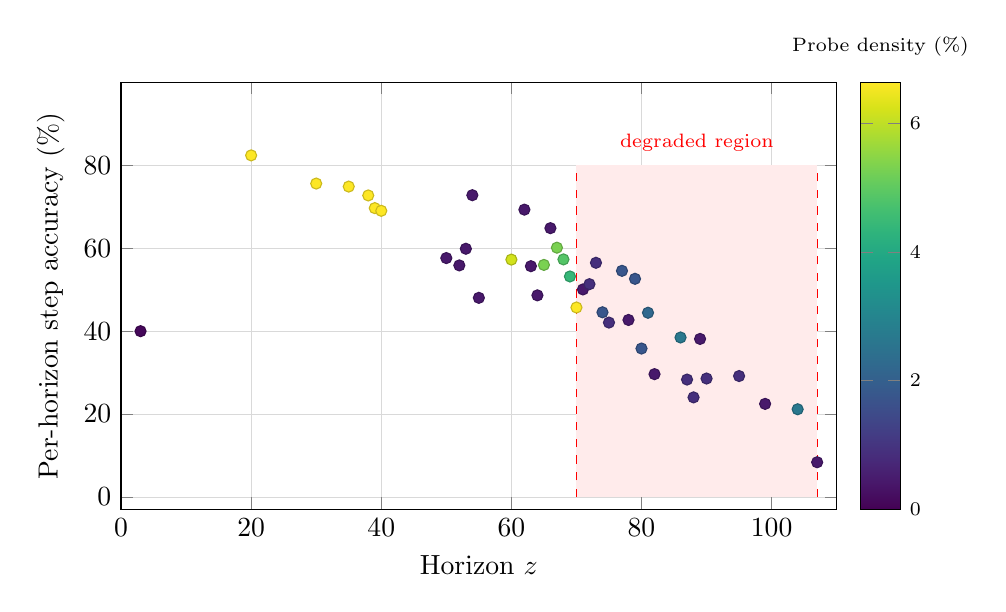
\begin{tikzpicture}
\begin{axis}[
    xlabel={Horizon $z$},
    ylabel={Per-horizon step accuracy (\%)},
    xmin=0, xmax=110,
    ymin=-3, ymax=100,
    width=0.88\linewidth,
    height=7cm,
    grid=both,
    major grid style={line width=.2pt,draw=gray!30},
    minor grid style={line width=.1pt,draw=gray!15},
    tick align=inside,
    xtick={0,20,40,60,80,100},
    ytick={0,20,40,60,80},
    legend style={font=\scriptsize, draw=none, at={(0.02,0.98)}, anchor=north west},
    scatter,
    only marks,
    mark=*,
    colormap/viridis,
    point meta min=0,
    point meta max=6.63,
    colorbar,
    colorbar style={
        title={Probe density (\%)},
        yticklabel style={font=\scriptsize},
        title style={font=\scriptsize},
    },
]
\path[fill=red!8] (axis cs:70,0) rectangle (axis cs:107,80);
\draw[red, dashed, thin] (axis cs:70,0) -- (axis cs:70,80);
\draw[red, dashed, thin] (axis cs:107,0) -- (axis cs:107,80);
\node[font=\scriptsize, text=red, anchor=south]
    at (axis cs:88.5,81) {degraded region};
\addplot[
    only marks,
    scatter,
    scatter src=explicit,
    mark=*,
] table[meta=density] {
z acc density
3 40.00 0.110
20 82.44 6.630
30 75.64 6.630
35 74.91 6.630
38 72.77 6.630
39 69.71 6.630
40 69.06 6.630
50 57.65 0.442
52 55.88 0.442
53 59.90 0.442
54 72.83 0.442
55 48.05 0.442
60 57.28 6.188
62 69.34 0.442
63 55.69 0.442
64 48.65 0.442
65 56.00 5.304
66 64.87 0.442
67 60.16 5.304
68 57.33 4.862
69 53.21 4.420
70 45.72 6.630
71 50.08 0.442
72 51.35 0.884
73 56.51 0.884
74 44.56 1.768
75 42.08 0.884
77 54.57 1.768
78 42.71 0.442
79 52.64 1.768
80 35.81 1.768
81 44.45 2.210
82 29.63 0.442
86 38.48 2.652
87 28.32 0.884
88 24.02 0.884
89 38.13 0.442
90 28.57 0.884
95 29.17 0.884
99 22.45 0.442
104 21.15 2.652
107 8.36 0.442
};


\end{axis}
\end{tikzpicture}
\caption{Pooled observed requested-$z$ Step Accuracy for Ministral 14B 2512, conditional on valid responses. Color encodes each horizon's share of all 4,525 recorded probes, including five calibration probes at $z=3$. The shaded $z=70$--107 region is an illustrative visual guide, not an estimated fracture interval or a claim that accuracy is monotonic.}
\label{fig:ministral_sampling_density}
\end{figure}

The density varies across sampled horizons. The shaded region highlights the later observed horizons without implying that all points fall below a fixed accuracy threshold. This descriptive plot does not establish the cause of the observed accuracy pattern.

\paragraph{Validity and MAI-Thinking-1 sampled horizons.}
In live AFS, the cognitive-validity filter excludes provider, infrastructure,
API, finish-reason, and classifier-invalid responses before computing batch accuracy.
An all-invalid batch returns no accuracy estimate and is treated as
insufficient evidence, so the adaptive search moves deeper rather than
recording a zero-accuracy fracture. The post-hoc fracture curve
similarly averages valid probes at each observed horizon and omits invalid-only
or missing horizons. Its two-point recovery check uses the next two
\emph{sampled} valid-curve points, not adjacent integer horizons; a candidate
without sufficient later support is right-censored. The validity gates are not
identical: live AFS checks explicit provider and infrastructure flags in
addition to classifier validity, whereas the post-hoc curve uses the
saved validity classification. Their Step Accuracy definitions also differ
from the requested-$z$ diagnostic above: the fracture curve uses the saved
full-transition metric, while that diagnostic scores the first $z$ reference
coordinates (the supplied initial state excluded).

For MAI-Thinking-1, every tier has 0 valid and 45 invalid responses at each of
$z=1,2,5,10$, so conditional accuracy is undefined there. The $z=20$ and
$z=30$ observations have high valid-conditional accuracy, as shown below.
On the valid-only curves,
Tiers 0, 2, and 3 have no fracture on the sampled support; Tier 1 has a
$z=150$ terminal candidate that is right-censored, not confirmed.

\begin{table}[H]
\centering
\caption{MAI-Thinking-1 sampled-horizon observations and valid-only fracture decisions. Accuracy is conditional on valid responses. The requested-$z$ metric and the saved full-transition metric use different coordinate conventions.}
\label{tab:mai_fracture_reconciliation}
\scriptsize
\setlength{\tabcolsep}{3.2pt}
\begin{tabular}{r c r r c c l}
\toprule
\textbf{$z$} & \textbf{Tier} & \textbf{Valid / total} & \textbf{Invalid} &
\textbf{Full-transition} & \textbf{Requested-$z$} & \textbf{Curve decision} \\
\midrule
1, 2, 5, 10 & Each & 0 / 45 & 45 & N/A & N/A &
No valid-curve point \\
20 & 0 & 29 / 76 & 47 & 98.97\% & 100.00\% &
None \\
20 & 1 & 29 / 76 & 47 & 98.97\% & 100.00\% &
$150^\dagger$ \\
20 & 2 & 30 / 76 & 46 & 99.17\% & 100.00\% &
None \\
20 & 3 & 29 / 75 & 46 & 99.83\% & 100.00\% &
None \\
30 & 0 & 61 / 75 & 14 & 98.85\% & 99.55\% &
None \\
30 & 1 & 64 / 75 & 11 & 97.29\% & 97.52\% &
$150^\dagger$ \\
30 & 2 & 55 / 75 & 20 & 98.00\% & 98.24\% &
None \\
30 & 3 & 60 / 75 & 15 & 99.56\% & 99.71\% &
None \\
\bottomrule
\end{tabular}
\end{table}

$^\dagger$Tier 1's terminal candidate is right-censored because the sampled
curve ends before a complete recovery window. Horizon gaps are not interpolated;
a missing or invalid-only horizon contributes no conditional-accuracy point.

\subsection{CRI}
\label{app:CRI}
The optional Composite Robustness Index (CRI) provides a secondary summary across evaluation axes:
 $\text{CRI} = 0.45\,\text{TF}
+0.30\,\text{HR}
+0.20\,\text{SR}
+0.05\,\text{GE}$.

Its components are:
\begin{enumerate}
    \item \textbf{Trajectory Fidelity}
    $\text{TF} = 0.5A + 0.3C + 0.2E$,
    where $A$ is step accuracy, $C$ is continuity, and $E$ is the requested-output exact-match rate.

    \item \textbf{Horizon Robustness}, defined as the normalized trapezoidal area under the accuracy-horizon curve:
    \[
    \text{HR} =
    \frac{
    \displaystyle\sum_i
    \frac{A_i+A_{i+1}}{2}
    (z_{i+1}-z_i)
    }{
    z_{\max}-z_{\min}
    }.
    \]

    \item \textbf{Semantic Robustness}
    $\text{SR} = 0.5R_1 + 0.25R_2 + 0.25R_3$,
    where $R_i=\min(1,A_i/A_0)$ is the ratio of Tier-$i$ accuracy to Tier-0 accuracy, clamped to $[0,1]$. If Tier-0 accuracy is zero or unavailable, SR is the arithmetic mean of the available tier accuracies. Tier 1 receives the larger weight because it is a label-only perturbation and leaves the transition function unchanged.
\end{enumerate}

\subsection{Seed-Level Variability}
\label{app:seed_variance}
Table~\ref{tab:cri_seed_variance} reports the population mean and standard
deviation of the secondary CRI across the five master seeds for each
run. These values characterize seed sensitivity; they are not
confidence intervals and should not be used to claim statistically significant
between-model differences.

\begin{table}[H]
\centering
\caption{CRI across five master seeds (population mean $\pm$ standard deviation). Asterisks indicate response validity below 75\%.}
\label{tab:cri_seed_variance}
\scriptsize
\begin{tabular}{lc}
\toprule
\textbf{Model} & \textbf{CRI} \\
\midrule
qwen.qwen3-235b-a22b-2507* & $0.250 \pm 0.027$ \\
Kimi K2.5 & $0.567 \pm 0.032$ \\
Qwen 3 Coder 480B A35B & $0.517 \pm 0.021$ \\
mistral-small-2603 & $0.505 \pm 0.023$ \\
Mistral Large 2512 & $0.538 \pm 0.016$ \\
mistral.devstral-2-123b* & $0.500 \pm 0.026$ \\
ministral-14b-2512 & $0.556 \pm 0.065$ \\
ministral-8b-2512 & $0.501 \pm 0.041$ \\
ministral-3b-2512 & $0.479 \pm 0.047$ \\
nvidia.nemotron-super-3-120b & $0.519 \pm 0.032$ \\
GLM-5 & $0.590 \pm 0.032$ \\
GPT-5-mini & $0.814 \pm 0.034$ \\
MAI-Thinking-1* & $0.480 \pm 0.049$ \\
\bottomrule
\end{tabular}
\end{table}

\subsection{Full Model Results}
\label{app:full_model}

\begin{table}[H]
\centering
\caption{Complete overall ARCUS-X results for all 13 evaluated models. Exact Match uses the requested $z$ coordinates and all completed probes. Asterisks indicate response validity below 75\%.}
\label{tab:overall_results_full}
\scriptsize
\resizebox{\linewidth}{!}{%
\begin{tabular}{lcccc}
\toprule
\textbf{Model} & \textbf{Step Acc.} & \textbf{Requested Exact Match} & \textbf{Continuity} & \textbf{Horizon Compliance} \\
\midrule
qwen.qwen3-235b-a22b-2507* & 14.1\% & 0.3\% & 11.9\% & 17.3\% \\
Kimi K2.5 & 59.2\% & 0.1\% & 53.9\% & 77.0\% \\
Qwen 3 Coder 480B A35B & 49.7\% & 1.2\% & 43.1\% & 98.3\% \\
mistral-small-2603 & 50.3\% & 0.6\% & 46.8\% & 80.1\% \\
Mistral Large 2512 & 56.0\% & 0.4\% & 53.0\% & 45.2\% \\
mistral.devstral-2-123b* & 44.7\% & 0.1\% & 43.3\% & 42.0\% \\
ministral-14b-2512 & 55.5\% & 5.9\% & 51.6\% & 74.5\% \\
ministral-8b-2512 & 47.7\% & 0.9\% & 45.0\% & 64.2\% \\
ministral-3b-2512 & 43.7\% & 8.4\% & 40.2\% & 72.7\% \\
nvidia.nemotron-super-3-120b & 47.7\% & 0.6\% & 42.4\% & 96.8\% \\
GLM-5 & 56.2\% & 1.0\% & 51.3\% & 98.4\% \\
GPT-5-mini & 85.3\% & 36.0\% & 85.0\% & 87.7\% \\
MAI-Thinking-1* & 40.0\% & 6.4\% & 40.0\% & 40.1\% \\
\bottomrule
\end{tabular}}
\end{table}

\subsubsection{Horizon-Dependent Degradation and Fracture}

\begin{figure}[H]
\centering
\includegraphics[width=\linewidth]{horizon_profiles.pdf}
\caption{Observed per-horizon accuracy for every evaluated model, pooled over all recorded non-calibration probes. Curves join only horizons sampled by the adaptive procedure.}
\label{fig:all_models_horizon_comparison}
\end{figure}

\begin{table}[H]
\centering
\caption{Post-hoc structural fracture depth by perturbation tier for all 13 evaluated models, using valid non-calibration responses only. Values are the first sampled horizon below the 50\% conditional Step Accuracy floor without recovery in the next two sampled horizons. `N/A' means that no persistent sampled fracture was found; $\dagger$ marks a terminal candidate with insufficient look-ahead and is not a confirmed fracture. Asterisks indicate response validity below 75\%.}
\label{tab:fracture_full}
\scriptsize
\begin{tabular}{lcccc}
\toprule
\textbf{Model} & \textbf{Tier 0} & \textbf{Tier 1} & \textbf{Tier 2} & \textbf{Tier 3} \\
\midrule
qwen.qwen3-235b-a22b-2507* & 18 & 12 & 23 & 12 \\
Kimi K2.5 & 145 & N/A & 130 & 55 \\
Qwen 3 Coder 480B A35B & 34 & 24 & 28 & 23 \\
mistral-small-2603 & 21 & 34$^\dagger$ & 20 & 17 \\
Mistral Large 2512 & 9 & 5 & 94 & 6 \\
mistral.devstral-2-123b* & 10 & 84 & 24 & 13 \\
ministral-14b-2512 & 69 & 99 & 80 & 40 \\
ministral-8b-2512 & 21 & 20 & 8 & 12 \\
ministral-3b-2512 & 22 & 28 & 25 & 27 \\
nvidia.nemotron-super-3-120b & 24 & 17 & 20 & 16 \\
GLM-5 & 57 & 44 & 56 & 30 \\
GPT-5-mini & N/A & N/A & N/A & N/A \\
MAI-Thinking-1* & N/A & 150$^\dagger$ & N/A & N/A \\
\bottomrule
\end{tabular}
\end{table}

The table reports the structural-yield analysis of the sampled valid-only curves, not an exhaustive scan of every integer horizon. The live AFS controller starts with an upper bound of $\min(40,H)$ and doubles that bound only after a passing (or operationally insufficient) midpoint reaches the current upper edge; expansion stops at the absolute hard ceiling $H=150$. We call the search window \emph{saturated} when no below-floor midpoint has been found and the lower search bound advances beyond $H$; the recorded live-search value is then the right-censored ceiling, $z=150$. This ceiling fallback is not evidence of 150-step cognitive survival, especially when batches are operationally insufficient. Conversely, the `N/A' entries above mean that the post-hoc two-point recovery rule found no persistent sampled fracture; they are not synonymous with a saturated live search. A dagger marks a terminal post-hoc candidate for which two future sampled horizons were unavailable.

\begin{table}[H]
\centering
\caption{Per-horizon accuracy fluctuation over observed horizons. Std. dev. is the population standard deviation of each model's per-horizon accuracies rounded to one decimal place. Asterisks indicate response validity below 75\%.}
\label{tab:horizon_fluctuation}
\scriptsize
\begin{tabular}{lccc}
\toprule
\textbf{Model} & \textbf{Observations ($N$)} & \textbf{Mean Accuracy} & \textbf{Std. Dev.} \\
\midrule
qwen.qwen3-235b-a22b-2507* & 43 & 16.90\% & 12.98\% \\
Kimi K2.5 & 64 & 55.75\% & 12.09\% \\
Qwen 3 Coder 480B A35B & 17 & 46.98\% & 7.41\% \\
mistral-small-2603 & 16 & 49.71\% & 11.26\% \\
Mistral Large 2512 & 61 & 50.24\% & 13.88\% \\
mistral.devstral-2-123b* & 73 & 36.84\% & 27.47\% \\
ministral-14b-2512 & 41 & 44.81\% & 20.61\% \\
ministral-8b-2512 & 38 & 46.01\% & 10.15\% \\
ministral-3b-2512 & 26 & 41.56\% & 16.30\% \\
nvidia.nemotron-super-3-120b & 16 & 46.88\% & 12.06\% \\
GLM-5 & 24 & 50.55\% & 9.67\% \\
GPT-5-mini & 19 & 85.33\% & 15.95\% \\
MAI-Thinking-1* & 55 & 41.61\% & 23.06\% \\
\bottomrule
\end{tabular}
\end{table}

\begin{table}[H]
\centering
\caption{Pearson correlation between horizon-accuracy fluctuation and trajectory-level metrics across all models.}
\label{tab:fluctuation_correlations}
\footnotesize
\begin{tabular}{lc}
\toprule
\textbf{Metric} & \textbf{Pearson $r$ with Fluctuation} \\
\midrule
Horizon Compliance & $-0.499$ \\
Exact Match & $0.172$ \\
Step Accuracy & $-0.060$ \\
Continuity & $0.023$ \\
\bottomrule
\end{tabular}
\end{table}

With only 13 model observations, these Pearson correlations are descriptive and exploratory rather than evidence of general population relationships. The fracture-depth correlation is omitted because fracture observations are right-censored at the search ceiling and absent for more than one model. Within this evaluation, greater fluctuation co-occurs with lower horizon compliance, while the relationships with step accuracy and continuity are near zero and exact match is weakly positive. These associations should not be interpreted as general claims about predictability beyond this sample.

\subsubsection{Semantic Robustness}

Table~\ref{tab:tier_full} reports per-tier step accuracy for all 13 evaluated models, since the benchmark runner evaluates all four tiers at every configured gravity value (Section~\ref{subsec:pert_regi}). Table~\ref{tab:cri_decomposition} reports the corresponding CRI decomposition, including the Semantic Robustness (SR) component (Appendix~\ref{app:CRI}).

\begin{table}[!ht]
\centering
\caption{Complete per-tier step accuracy for all 13 evaluated models. Asterisks indicate response validity below 75\%.}
\label{tab:tier_full}
\scriptsize
\begin{tabular}{lcccc}
\toprule
\textbf{Model} & \textbf{Tier 0} & \textbf{Tier 1} & \textbf{Tier 2} & \textbf{Tier 3} \\
\midrule
qwen.qwen3-235b-a22b-2507* & 17.2\% & 15.1\% & 19.0\% & 5.2\% \\
Kimi K2.5 & 63.1\% & 75.8\% & 65.2\% & 32.9\% \\
Qwen 3 Coder 480B A35B & 56.9\% & 49.7\% & 53.7\% & 38.4\% \\
mistral-small-2603 & 47.7\% & 63.3\% & 46.6\% & 43.8\% \\
Mistral Large 2512 & 56.1\% & 48.6\% & 58.6\% & 60.5\% \\
mistral.devstral-2-123b* & 44.7\% & 52.3\% & 44.4\% & 37.3\% \\
ministral-14b-2512 & 56.2\% & 60.9\% & 55.8\% & 49.0\% \\
ministral-8b-2512 & 48.4\% & 47.0\% & 45.3\% & 50.3\% \\
ministral-3b-2512 & 43.3\% & 44.3\% & 42.7\% & 44.3\% \\
nvidia.nemotron-super-3-120b & 56.8\% & 45.4\% & 50.7\% & 37.9\% \\
GLM-5 & 64.5\% & 58.7\% & 60.3\% & 41.3\% \\
GPT-5-mini & 88.0\% & 83.7\% & 87.5\% & 82.2\% \\
MAI-Thinking-1* & 45.0\% & 29.1\% & 46.7\% & 39.2\% \\
\bottomrule
\end{tabular}
\end{table}

\begin{table}[!ht]
\centering
\caption{CRI and its decomposition for all 13 evaluated models: Trajectory Fidelity (TF), Horizon Robustness (HR), Semantic Robustness (SR), and Generation Efficiency (GE), pooled across probes (Appendix~\ref{app:CRI}). Asterisks indicate response validity below 75\%.}
\label{tab:cri_decomposition}
\scriptsize
\begin{tabular}{lccccc}
\toprule
\textbf{Model} & \textbf{TF} & \textbf{HR} & \textbf{SR} & \textbf{GE} & \textbf{CRI} \\
\midrule
qwen.qwen3-235b-a22b-2507* & 0.107 & 0.073 & 0.764 & 0.823 & 0.264 \\
Kimi K2.5 & 0.458 & 0.498 & 0.880 & 0.559 & 0.559 \\
Qwen 3 Coder 480B A35B & 0.380 & 0.404 & 0.841 & 0.994 & 0.510 \\
mistral-small-2603 & 0.393 & 0.296 & 0.973 & 0.603 & 0.491 \\
Mistral Large 2512 & 0.440 & 0.502 & 0.933 & 0.238 & 0.547 \\
mistral.devstral-2-123b* & 0.353 & 0.306 & 0.957 & 0.551 & 0.470 \\
ministral-14b-2512 & 0.444 & 0.381 & 0.967 & 0.361 & 0.525 \\
ministral-8b-2512 & 0.375 & 0.364 & 0.969 & 0.266 & 0.485 \\
ministral-3b-2512 & 0.356 & 0.343 & 0.997 & 0.214 & 0.473 \\
nvidia.nemotron-super-3-120b & 0.367 & 0.547 & 0.790 & 0.999 & 0.537 \\
GLM-5 & 0.437 & 0.535 & 0.848 & 1.000 & 0.577 \\
GPT-5-mini & 0.754 & 0.836 & 0.958 & 0.256 & 0.794 \\
MAI-Thinking-1* & 0.333 & 0.436 & 0.790 & 0.700 & 0.474 \\
\bottomrule
\end{tabular}
\end{table}

The CRI values in Table~\ref{tab:cri_decomposition} are pooled single-run summaries and differ slightly from the per-seed population means reported in Appendix~\ref{app:seed_variance}, which average five independently computed CRI values per model. The two summaries are not interchangeable: the pooled CRI aggregates all probes as a single sample, while the seed-level mean averages five separately computed run-level statistics.

\subsection{Generation Efficiency and Failure Modes}

\begin{table}[!ht]
\centering
\caption{Generation efficiency measurements. Asterisks indicate response validity below 75\%.}
\label{tab:generation_efficiency}
\scriptsize
\begin{tabular}{lcccc}
\toprule
\textbf{Model} & \textbf{Step Accuracy} & \textbf{GBI} & \textbf{Generation Efficiency} & \textbf{Correct Steps/sec} \\
\midrule
qwen.qwen3-235b-a22b-2507* & 14.1\% & 1.44 & 82.3\% & 0.283 \\
Kimi K2.5 & 59.2\% & 1.12 & 55.9\% & 2.406 \\
Qwen 3 Coder 480B A35B & 49.7\% & 0.02 & 99.4\% & 6.786 \\
mistral-small-2603 & 50.3\% & 1.58 & 60.3\% & 3.083 \\
Mistral Large 2512 & 56.0\% & 4.49 & 23.8\% & 1.127 \\
mistral.devstral-2-123b* & 44.7\% & 1.91 & 55.1\% & 1.131 \\
ministral-14b-2512 & 55.5\% & 2.39 & 36.1\% & 1.411 \\
ministral-8b-2512 & 47.7\% & 3.33 & 26.6\% & 0.930 \\
ministral-3b-2512 & 43.7\% & 4.91 & 21.4\% & 1.543 \\
nvidia.nemotron-super-3-120b & 47.7\% & 0.03 & 99.9\% & 4.278 \\
GLM-5 & 56.2\% & 0.00 & 100.0\% & 4.626 \\
GPT-5-mini & 85.3\% & 4.25 & 25.6\% & 1.922 \\
MAI-Thinking-1* & 40.0\% & 1.41 & 70.0\% & 0.694 \\
\bottomrule
\end{tabular}
\end{table}

Table~\ref{tab:failure_taxonomy_full} reports the complete validity and taxonomy partition for all 13 evaluated models, extending the five-model view in Table~\ref{tab:failure_taxonomy_selected}. Figure~\ref{fig:failure_profiles} visualizes the five primary failure categories; \emph{None}, Unknown / Unmapped, and invalid responses remain visible in the table rather than the heatmap.

\begin{table}[!ht]
\centering
\caption{Post-run validity and requested-output taxonomy partition for the 13-model cohort. Taxonomy percentages are relative to valid probes; \emph{None} is requested-output Exact Match. Invalid responses are reported separately.}
\label{tab:failure_taxonomy_full}
\scriptsize
\resizebox{\linewidth}{!}{%
\begin{tabular}{lccccccccc}
\toprule
\textbf{Model} & \textbf{Valid} & \textbf{Invalid} & \textbf{State} & \textbf{Transition} & \textbf{Semantic} & \textbf{Horizon} & \textbf{Format} & \textbf{Unknown} & \textbf{None} \\
\midrule
qwen.qwen3-235b-a22b-2507* & 26.0\% & 74.0\% & 8.2\% & 2.0\% & 37.2\% & 40.2\% & 11.0\% & 0.0\% & 1.3\% \\
Kimi K2.5 & 94.8\% & 5.2\% & 10.7\% & 4.0\% & 23.2\% & 56.1\% & 5.9\% & 0.0\% & 0.1\% \\
Qwen 3 Coder 480B A35B & 100.0\% & 0.0\% & 94.0\% & 1.1\% & 0.0\% & 3.6\% & 0.0\% & 0.0\% & 1.2\% \\
mistral-small-2603 & 100.0\% & 0.0\% & 47.8\% & 17.6\% & 0.3\% & 33.5\% & 0.0\% & 0.0\% & 0.6\% \\
Mistral Large 2512 & 96.9\% & 3.1\% & 11.1\% & 24.8\% & 10.2\% & 49.4\% & 4.1\% & 0.0\% & 0.4\% \\
mistral.devstral-2-123b* & 72.7\% & 27.3\% & 23.7\% & 23.9\% & 0.7\% & 50.9\% & 0.8\% & 0.0\% & 0.1\% \\
ministral-14b-2512 & 91.2\% & 8.8\% & 50.6\% & 11.1\% & 1.3\% & 29.9\% & 0.7\% & 0.0\% & 6.4\% \\
ministral-8b-2512 & 99.7\% & 0.3\% & 21.2\% & 40.4\% & 0.3\% & 36.8\% & 0.4\% & 0.0\% & 0.9\% \\
ministral-3b-2512 & 82.0\% & 18.0\% & 56.9\% & 4.6\% & 6.4\% & 16.2\% & 5.7\% & 0.1\% & 10.2\% \\
nvidia.nemotron-super-3-120b & 99.9\% & 0.1\% & 92.6\% & 1.1\% & 0.0\% & 5.4\% & 0.2\% & 0.0\% & 0.6\% \\
GLM-5 & 100.0\% & 0.0\% & 84.3\% & 0.6\% & 0.0\% & 14.2\% & 0.0\% & 0.0\% & 1.0\% \\
GPT-5-mini & 88.8\% & 11.2\% & 10.4\% & 0.1\% & 0.0\% & 49.0\% & 0.0\% & 0.0\% & 40.5\% \\
MAI-Thinking-1* & 40.8\% & 59.2\% & 3.0\% & 0.0\% & 0.0\% & 81.2\% & 0.0\% & 0.0\% & 15.8\% \\
\bottomrule
\end{tabular}}
\end{table}

\begin{figure}[H]
\centering
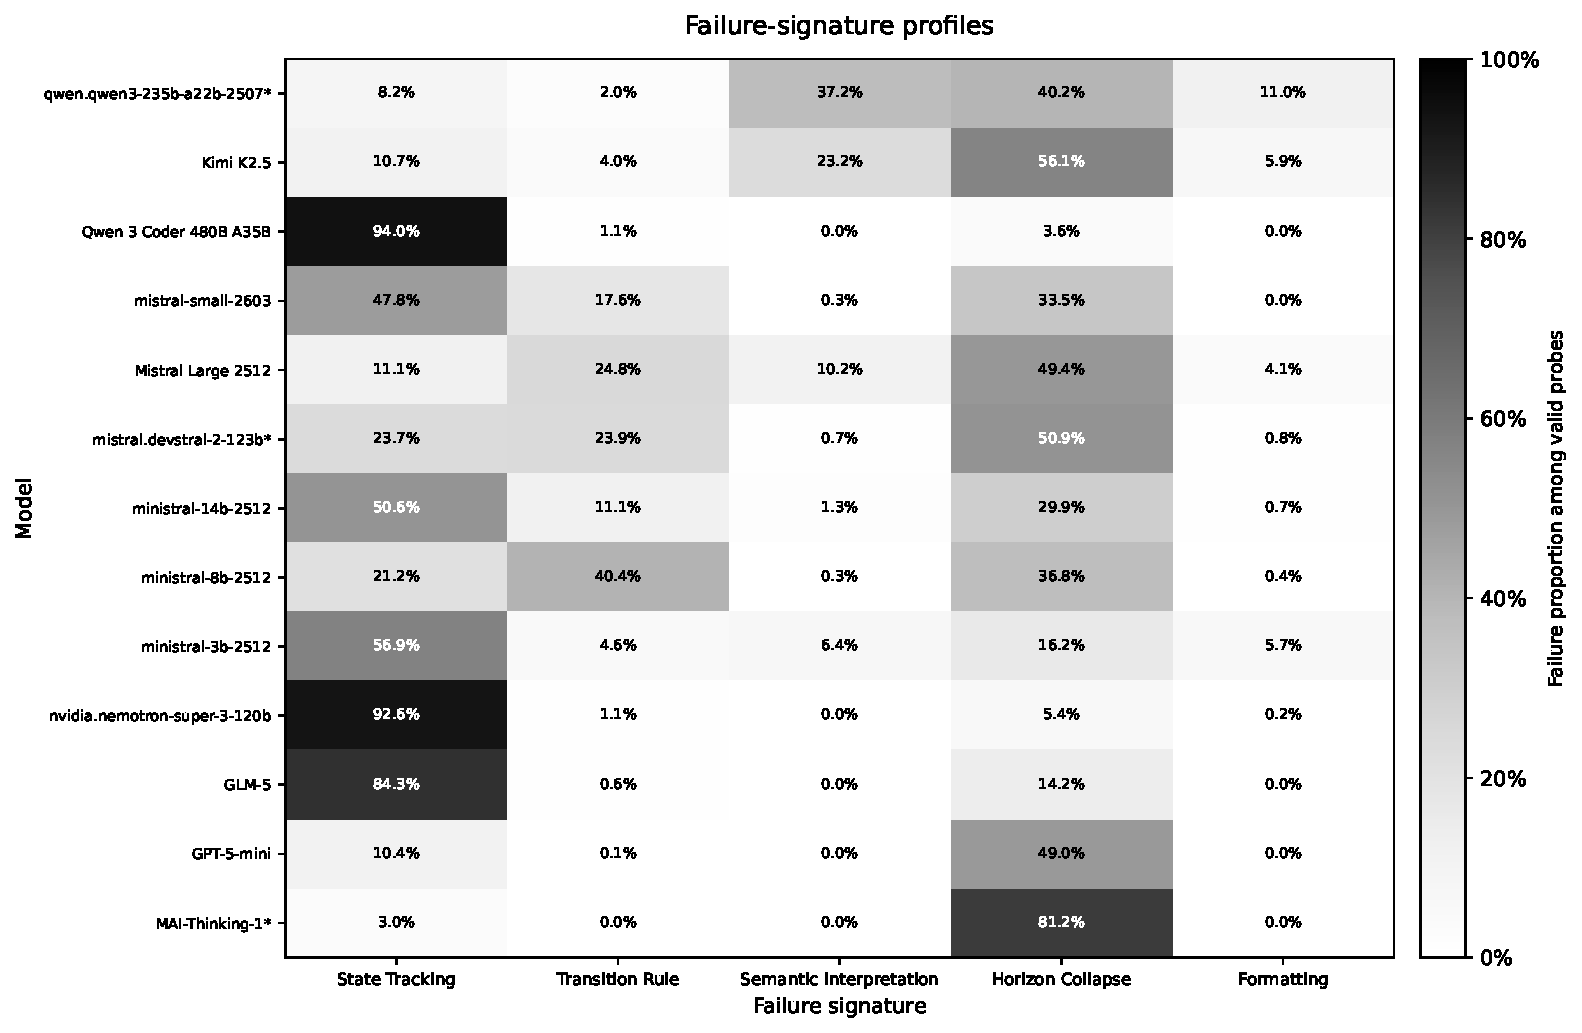
\includegraphics[width=\linewidth]{failure_profiles_requested.pdf}
\caption{Failure-signature profiles across the 13-model publication cohort, expressed as a percentage of valid probes. Asterisks in the row labels identify models with response validity below 75\%.}
\label{fig:failure_profiles}
\end{figure}

For models with low response validity, the taxonomy columns describe only the analyzable subset and may therefore be less representative of all completed probes.

\subsection{Taxonomy Policy Sensitivity}
\label{app:taxonomy_sensitivity}
The requested-output taxonomy is the primary analysis. We vary one policy at a time without replacing the primary labels. Across 39,728 valid non-calibration observations, horizon-first reassigns 34.4\% and transition-first 33.6\%; modulo sensitivity reassigns 0.013\%, while conservative and fallback-as-State policies reassign 0.010\% and 0.008\%, respectively. The table reports the percentage of valid observations whose primary label changes. The conservative policy maps unknown cases to Unclassified; fallback-as-State assigns early divergences without an explicit mapped mechanism to State Tracking; horizon-first and transition-first reorder the corresponding detected indicator; modulo sensitivity treats requested-length modulo-equivalent noncanonical paths as correct. Sensitivity counts are retained in the reproducibility artifacts.
\begin{table}[!ht]
\centering
\caption{Share of valid probes reassigned relative to the primary taxonomy under alternative policies.}
\label{tab:taxonomy_policy_stability}
\scriptsize
\resizebox{\linewidth}{!}{%
\begin{tabular}{lccccc}
\toprule
\textbf{Model} & \textbf{Conservative} & \textbf{Fallback as State} & \textbf{Horizon-first} & \textbf{Transition-first} & \textbf{Modulo} \\
\midrule
qwen.qwen3-235b-a22b-2507* & 0.0\% & 0.0\% & 54.1\% & 7.7\% & 0.0\% \\
Kimi K2.5 & 0.0\% & 0.0\% & 42.6\% & 10.5\% & 0.0\% \\
Qwen 3 Coder 480B A35B & 0.0\% & 0.0\% & 28.6\% & 92.3\% & 0.0\% \\
mistral-small-2603 & 0.0\% & 0.0\% & 30.7\% & 47.7\% & 0.0\% \\
Mistral Large 2512 & 0.0\% & 0.0\% & 49.3\% & 11.0\% & 0.0\% \\
mistral.devstral-2-123b* & 0.0\% & 0.0\% & 46.0\% & 23.3\% & 0.0\% \\
ministral-14b-2512 & 0.0\% & 0.0\% & 39.7\% & 50.3\% & 0.0\% \\
ministral-8b-2512 & 0.0\% & 0.0\% & 59.3\% & 20.5\% & 0.0\% \\
ministral-3b-2512 & 0.1\% & 0.1\% & 34.6\% & 55.5\% & 0.2\% \\
nvidia.nemotron-super-3-120b & 0.0\% & 0.0\% & 45.8\% & 90.8\% & 0.0\% \\
GLM-5 & 0.0\% & 0.0\% & 39.1\% & 80.8\% & 0.0\% \\
GPT-5-mini & 0.0\% & 0.0\% & 2.8\% & 10.4\% & 0.0\% \\
MAI-Thinking-1* & 0.0\% & 0.0\% & 2.5\% & 2.9\% & 0.0\% \\
\bottomrule
\end{tabular}}
\end{table}


\subsection{Synthetic Sampling-Efficiency Evaluation}
\label{app:afs_simulation}
We compared the production AFS controller with fixed-grid, sequential, uniform-random, and threshold-directed adaptive sampling on synthetic accuracy and validity curves, without model inference. The test set contains 200 independently parameterized curves in each of nine families and two noise realizations per curve. Each policy pays for one calibration response and five responses per sampled horizon; invalid responses consume budget but are excluded from batch accuracy. Valid probe scores follow a beta-binomial model of the $z$ transition positions. The estimand is the first integer horizon with conditional accuracy below 50\%; a common estimator uses the earliest sampled valid batch below that threshold. A five-consecutive-horizon target and alternative thresholds are examined separately. The complete generating curve is available only to the evaluator.

\begin{table}[H]
\centering
\caption{Synthetic first-crossing performance at an 81-response budget. Within-five and detection rates are conditional on a true crossing; brackets give curve-clustered 95\% intervals. Mean absolute error (MAE) is conditional on detection. False-positive rates are conditional on no true crossing.}
\label{tab:afs_simulation}
\scriptsize
\begin{tabular}{lrrrr}
\toprule
Policy & Within five & Detected & MAE & False positive \\
\midrule
Production AFS & 59.3\% [57.3\%, 61.4\%] & 94.0\% & 9.59 & 31.2\% \\
Fixed grid & 46.5\% [44.5\%, 48.5\%] & 94.4\% & 11.40 & 38.9\% \\
Sequential & 16.7\% [14.7\%, 18.7\%] & 28.5\% & 21.88 & 37.1\% \\
Uniform random & 37.8\% [36.3\%, 39.7\%] & 92.1\% & 13.24 & 33.7\% \\
Adaptive alternative & 42.0\% [39.8\%, 44.3\%] & 95.3\% & 22.12 & 46.3\% \\
\bottomrule
\end{tabular}
\end{table}

At this budget, AFS localized 59.3\% of pooled crossings within five horizons, compared with 46.5\% for the fixed grid (paired difference 12.8 percentage points, 95\% CI [10.1, 15.4]). In the recovery family the respective rates were 91.0\% and 58.0\%; in the oscillatory family they were 37.5\% and 62.3\%. The persistent estimator detected 0 of 3096 realizations with a true persistent crossing under AFS at this budget; it requires five consecutively sampled valid below-threshold horizons. These are synthetic allocation results, not estimates of empirical LLM sample efficiency. The pooled rates depend on the chosen family mixture and response model; AFS may terminate with unused budget. Curve-clustered paired intervals, actual-cost comparisons, persistent-crossing results, validity and correlation stress tests, and family-specific outcomes are reported in the supplementary reproducibility artifacts. Lack of an observed crossing is not proof of no fracture.

\section{Minitest transcripts}
These are the recorded prompts, model responses, and reference trajectories for
Ministral-14B-2512 at $z=50$, seed 3157, and gravity 0.5 across all four tiers.
The prompts are reproduced as sent.
\IfFileExists{minitests_ministral-14b-2512_transcripts.txt}
  {\VerbatimInput[breaklines,breakanywhere,fontsize=\scriptsize]{minitests_ministral-14b-2512_transcripts.txt}}
  {\noindent\emph{Transcript file not included in this source package.}}

\noindent\textbf{Reference and scoring convention.}
The deterministic environment retains the complete
ground-truth trajectory of $z+1$ states for $z$
generated actions, including the initial state.
Because the model-facing prompt explicitly requests
$z$ output coordinates, post-hoc trajectory scoring
uses the first $z$ reference coordinates.
The initial coordinate is excluded from Step Accuracy
and Continuity, leaving $z-1$ scored post-initial
positions. The full $z+1$-state reference is
preserved for reproducibility and auditing.

\paragraph{Worked evaluation example.}
Consider the Tier~0 Ministral-14B-2512 probe at
$z=50$, with initial state $(2,7)$ on a
$5\times 8$ toroidal grid. Under the requested
output convention, the evaluated trajectory
contains $z=50$ coordinates, including the
initial state, and therefore $z-1=49$ scored
post-initial positions.

The model produces 50 coordinates. Its first
disagreement with the reference occurs at
coordinate 13 (one-indexed), corresponding
to the state after the twelfth action:
the model outputs $(2,0)$, whereas the
reference specifies $(3,7)$.

Comparing the model output against the first
50 coordinates of the recorded reference
gives 21 correct post-initial positions.
Consequently, Step Accuracy is
\[
    \mathrm{SA}=\frac{21}{49}\approx 0.429.
\]
The first 11 post-initial positions are
correct, giving Continuity
\[
    \mathrm{C}=\frac{11}{49}\approx 0.224.
\]
Because the trajectories differ, Exact Match
is zero. The model produces the requested
50 coordinates, yielding Horizon Compliance
\[
    \mathrm{HC}
    =1-\frac{|50-50|}{\max(50,50)}
    =1.
\]
Thus, compliance with the requested output
length does not imply correct sequential
execution.

\end{document}
